\documentclass{article}

\usepackage{amsmath, amsthm, amssymb, amsfonts}
\usepackage{thmtools}
\usepackage{graphicx}
\usepackage{setspace}
\usepackage{geometry}
\usepackage{float}
\usepackage{hyperref}
\usepackage[utf8]{inputenc}
\usepackage[spanish]{babel}
\usepackage{framed}
\usepackage[dvipsnames]{xcolor}
\usepackage{tcolorbox}
\usepackage{titlesec}
\usepackage{fancyhdr}
\usepackage{newclude}
\usepackage{pgfplots}
\usepackage{tikz}
\usepackage{enumitem}
\usepackage{bookmark}
\usepackage{bbm}

\pgfplotsset{compat=1.18}

\colorlet{LightGray}{White!90!Periwinkle}
\colorlet{LightOrange}{Orange!15}
\colorlet{LightGreen}{Green!15}

\newcommand{\HRule}[1]{\rule{\linewidth}{#1}}

\declaretheoremstyle[name=Teorema,]{thmsty}
\declaretheorem[style=thmsty,numberwithin=section]{theorem}
\tcolorboxenvironment{theorem}{colback=LightGray}

\declaretheoremstyle[name=Ejercicio,]{prosty}
\declaretheorem[style=prosty,numberlike=theorem]{exercise}
\tcolorboxenvironment{exercise}{colback=LightOrange}

\declaretheoremstyle[name=Demostración,]{prcpsty}
\declaretheorem[style=prcpsty,numberlike=theorem]{proofs}
\tcolorboxenvironment{proofs}{colback=LightGreen}

\declaretheoremstyle[name={..}, numbered=no,]{prcpsty_nonum}
\declaretheorem[style=prcpsty_nonum,unnumbered]{proofs*} % Unnumbered version
\tcolorboxenvironment{proofs*}{colback=LightGreen}

\pgfmathdeclarefunction{gauss}{2}{\pgfmathparse{1/(#2*sqrt(2*pi))*exp(-((x-#1)^2)/(2*#2^2))}}

\setstretch{1.2}
\geometry{
    textheight=9in,
    textwidth=5.5in,
    top=1in,
    headheight=12pt,
    headsep=25pt,
    footskip=30pt
}
    
\newenvironment{sectionpage}[2]{
    \clearpage

    \refstepcounter{section}
    \addcontentsline{toc}{section}{\thesection\quad #1: #2}
    \begin{center}
        \Huge \textbf{#1}\\
        \vspace{0.5em}
        \Large\textit{#2}
    \end{center}
    \vspace{1em}
    \hrule height 1pt
    \vspace{1em}
}{
    \vspace{1em}
    \hrule height 1pt
    \vfill
}

% ------------------------------------------------------------------------------

\begin{document}

% ------------------------------------------------------------------------------
% Cover Page and ToC
% ------------------------------------------------------------------------------

\title{ \normalsize \textsc{}
    \\ [2.0cm]
    \HRule{1.5pt} \\
    \LARGE \textbf{\uppercase{Inferencia Estadística II}
    \HRule{2.0pt} \\ [0.6cm] \LARGE{Apuntes de la asignatura} \vspace*{10\baselineskip}}
}

\author{\textbf{Autores} \\
    Victor Elvira Fernández, Tomás Ruiz Rojo, Juan Horrillo Crespo \\
    Universidad de Valladolid \\
    \date{\today}}

\maketitle
\newpage

\begin{center}
    \Huge \textbf{AVISO}
\end{center}

Estos apuntes fueron creados de forma voluntaria por un grupo de estudiantes, invirtiendo tiempo, dedicación y esfuerzo para ofrecer información útil a la comunidad. Apreciamos cualquier apoyo que se nos quiera brindar, ya que nos ayuda a continuar con futuros proyectos de este tipo. \\

Si deseas colaborar en esta clase de proyectos puedes contactarnos y unirte o invitarnos a unas ricas patatas 5 salsas por el siguiente enlace:

\vfil

\begin{center}
    \href{https://www.buymeacoffee.com/ApuntesINdat}{\LARGE \textbf{Buy Me a Patatas 5 Salsas}}
    \href{https://www.buymeacoffee.com/ApuntesINdat}{https://www.buymeacoffee.com/ApuntesINdat}
\end{center}

\begin{itemize}
    \item \href{mailto:juan.horrillo22@estudiantes.uva.es}{Mail Juan Horrillo}
    \item \href{mailto:victor.elvira22@estudiantes.uva.es}{Mail Victor Elvira}
    \item \href{mailto:tomas.rojo22@estudiantes.uva.es}{Mail Tomás Rojo}
\end{itemize}

\vfil

Si has colaborado de cualquier forma te agradecemos enormemente.

\tableofcontents
\newpage

% ------------------------------------------------------------------------------

\begin{sectionpage}{Tema 1}{Propiedades asintóticas del EMV y del estadístico RV}
    Uso y propiedades asintóticas del estimador de máxima verosimilitud (EMV) y del estadístico de razón de verosimilitud (RV).
\end{sectionpage}

\section{Estimadores en muestras grandes}

Sean $X_1, X_2, \dots, X_n$ variables aleatorias independientes igualmente distribuidas (v.a.i.i.d.) tal que $P_\theta:\theta \in \Theta$. Tenemos nuestra muestra aleatoria simple (m.a.s) con $n$ grande y nos interesa estimar $\theta$ (o $g(\theta)$).

Cuando el tamaño de la muestra aumenta, también aumenta la información disponible de $\theta$ (o $g(\theta)$), por lo tanto se espera que la estimación sea más precisa. Esto podemos comprobarlo al analizar la distribución de la media muestral ya que como $\overline{X}\thicksim N\left(\mu, \frac{\sigma^2}{n}\right)$, entonces $Var(\overline{X}) \xrightarrow{n \rightarrow \infty} 0$.

\begin{figure}[h!]
    \begin{center}
        \begin{tikzpicture}
            \begin{axis}[no markers, domain=0:10, samples=100, axis lines*=left, xlabel=Test,
                    ylabel=, height=6cm, width=10cm, enlargelimits=false, clip=false, axis on top,
                    grid = major,legend style={at={(0.5,-0.1)},anchor=north, legend columns=-1}]

                \addplot [fill=cyan!20, draw=blue, domain=-4:4] {gauss(0,0.6)} \closedcycle;
                \addlegendentry{N(0,0.8)}
                \addplot [fill=orange!20, fill opacity=0.5, draw=red, domain=-4:4] {gauss(0,1)} \closedcycle;
                \addlegendentry{N(0,1)}
            \end{axis}
        \end{tikzpicture}
        \caption{Comparación aumento de n}
    \end{center}
\end{figure}

Consideraremos que un estimador $T(X_1, \dots, X_n)$ es razonable si cuando $n$ aumenta, el estimador $T(X_1, \dots, X_n)$ es más preciso. Lo que podemos esperar es que $T(X_1, \dots, X_n)$ esté próximo a $\theta$ con mayor probabilidad. \\

A continuación, se definirán los criterios que nos permitirán comprobar la calidad de información que nos proporciona un estimador.

\subsection{Consistencia de un estimador}

Se dice que un estimador $T(X_1,\dots,X_n)$ es consistente si cumple que

\[
    \forall \varepsilon > 0, \delta > 0 \quad \exists N: n \geq N
\]
\[
    P_\theta(|T(X_1, \dots, X_n) - \theta| < \varepsilon) \geq 1 - \delta
\]

\textbf{\textit{Definición: }} $T_n(X)$ es un estimador consistente para $\theta$ (o $g(\theta)$) si

\[
    \forall \varepsilon > 0 \quad P_\theta\left(|T(X_1, \dots, X_n) - \theta| \leq \varepsilon\right) \xrightarrow{n \to \infty} 1
\]

es decir, si:

\[
    T_n(x) \overset{p}{\underset{n \to \infty}{\to}} \theta \quad \text{o} \quad \lim_{n \to \infty} \forall \varepsilon > 0 \quad P_\theta(|T(X_1, \dots, X_n) - \theta| \leq \varepsilon) = 1
\]

\newpage

Existen algunas estrategias para comprobar si un estimador es consistente:
\begin{enumerate}
    \item \textbf{Convergencia en probabilidad}. Si $T_n(x) \overset{p}{\underset{n \to \infty}{\to}} \theta$ y $G_n(x) \overset{p}{\underset{n \to \infty}{\to}} \theta'$
          \begin{itemize}
              \item $T_n(x)+G_n(x) \overset{p}{\underset{n \to \infty}{\to}} \theta + \theta '$
              \item $T_n(x) \cdot G_n(x) \overset{p}{\underset{n \to \infty}{\to}} \theta \cdot \theta '$
              \item Si $\theta' \neq 0, \frac{T_n(x)}{G_n(x)} \overset{p}{\underset{n \to \infty}{\to}} \frac{\theta}{\theta '}$
          \end{itemize}

    \item \textbf{Ley débil de los grandes números}. $X_1, X_2, \dots, X_n$ i.i.d. con $E(X_i)=\mu < \infty$
          \[\frac{1}{n}\sum_{i=1}^{n} X_i \overset{p}{\underset{n \to \infty}{\to}} \mu\]
          Los momentos muestrales son estimaciones consistentes de los correspondientes momentos poblacionales.

    \item \textbf{Convergencia en media cuadrática}. Un estimador $T(X_1, \dots, X_n)\xrightarrow{\underset{n \to \infty}{\text{m.c.}}} \theta$ si:
          \begin{itemize}
              \item $E(T(X_1, \dots, X_n)) \xrightarrow{{n \to \infty}} \theta$, sesgo de $T(X_1, \dots, X_n)\xrightarrow{{n \to \infty}} 0$
              \item $Var(T(X_1, \dots, X_n)) \xrightarrow{{n \to \infty}} 0$
          \end{itemize}
          Es decir que si ECM $T(X_1, \dots, X_n) \xrightarrow{{n \to \infty}} 0$, el estimador converge en media cuadrática. Un estimador insesgado sería consistente si su varianza converge a 0 con $n \to \infty$. La convergencia en media cuadrática es más fuerte que la convergencia en probabilidad.
\end{enumerate}

\begin{exercise}
    Sean $X_1, \dots, X_n$ v.a.i.i.d. con $E(X_i)=\mu$ y $Var(X_i)=\sigma^2$, $\forall i=1, \dots, n$. ¿Es consistente $T_n(x) = \frac{X_1 + X_2 + \dotsb + X_n}{\frac{n}{2}}$?

    Usando la ley de los grandes números:
    \[
        \frac{1}{n}\sum X_i \xrightarrow{\text{P}} \mu \quad T_n(x)\xrightarrow{P}2\mu
    \]

    Resultado: El estimador $T_n(x)$ NO es consistente
\end{exercise}

La consistencia por si sola no es tan interesante, ya que si $T_n$ es consistente para $\theta$, nos dice que para n grande los errores serán pequeños pero no nos permite conocer el orden del error $\left(\frac{1}{n}, \frac{1}{\sqrt{n}},\frac{1}{\log(n)}, \dots\right)$

Si $\{K_n\}_{n=1}^{\infty}$ es una sucesión de reales positivos y $\varepsilon>0$ definimos $P_n(\varepsilon)$ como

\[P_n(\varepsilon)=P_\theta\left(|T_n(x)-\theta| \leq \frac{\varepsilon}{K_n}\right)\]

Habiendo definido $P_n(\varepsilon)$, ¿qué pasará con $P_n(\varepsilon)$ cuando $n$ sea grande?
\begin{enumerate}
    \item Si $K_n$ crece "lentamente" (por ejemplo:  $K_n=\log(n)$), el error disminuye "lentamente" a medida que aumenta n $P_n(\varepsilon) \xrightarrow{{\text{n} \to \infty}} 1$. Si $K_n$ crece lentamente, $ \frac{\varepsilon}{K_n}$ es más grande, lo que facilitará que el error esté por debajo del umbral.
    \item Si $K_n$ crece "rápido" (por ejemplo:  $K_n=n$), el error disminuye más rápido a medida que aumenta n $P_n(\varepsilon) \xrightarrow{{\text{n} \to \infty}} 0$.  Si $K_n$ crece rápido, $ \frac{\varepsilon}{K_n}$ se hace muy pequeño y se hace muy difícil que el error sea tan pequeño.
    \item Casos intermedios. Si $K_n$ crece "adecuadamente", $P_n(\varepsilon) \xrightarrow{{\text{n} \to \infty}} H(\varepsilon) \in (0,1)$. Decimos que el error converge a 0 a velocidad $\frac{1}{K_n}$
\end{enumerate}

De manera resumida:

\[
    P_n(\varepsilon) = P_\theta(K_n|T_n(x) - \theta| \leq \varepsilon) \xrightarrow{n \to \infty}\begin{Bmatrix}
        0 \text{ si } K_n \xrightarrow{\infty} \text{rápido}                                  \\
        0 \leq P_n(\varepsilon) \leq 1 \text{ si } K_n \xrightarrow{\infty} \text{adecuadamente} \\
        1 \text{ si } K_n \xrightarrow{\infty} \text{lento}
    \end{Bmatrix}
\]

La idea es que al multiplicar $K_n$, se amplifica la velocidad de convergencia de los errores a 0. Si elegimos $K_n$ adecuadamente, de forma que $P_n(\varepsilon)$ sea menor que 1, podemos controlar la velocidad a la que los errores tienden a 0, mejorando la precisión.

\subsection{Estimador Consistente Asintoticamente Normal (CAN)}

\textbf{\textit{Definición: }} Sean $X_1,\dots,X_n$ v.a.i.i.d. con distribución $P_\theta$ donde $\theta \in \Theta$, entonces un estimador $T_n(X)=T(X_1,\dots,X_n)$ con $n\geq 1$ será CAN para $\theta$ si

\[
    \exists \sigma_n(\theta) > 0, \theta \xrightarrow{n\to\infty}0 \quad \text{tal que}\quad \frac{T_n(X)-\theta}{\sigma_n(\theta)}\overset{L}{\to}N(0,1)
\]

En muchas ocasiones, $\sigma^2_n(\theta)$ es de la forma $\frac{Var_\theta(T_n(X))}{n}$ y se llama varianza asintótica del estimador. En este caso $T_n(X)$ es CAN para $\theta$ si

\[
    \sqrt{n}(|T_n(X)-\theta|) \overset{L}{\to} N(0, Var_\theta(T_n(X)))
\]

donde los errores convergen a 0 con velocidad $\frac{1}{\sqrt{n}}$.

Al igual que la LGN es clave para obtener estimadores consistentes, el TCL lo es para obtener estimadores CAN. \\
Sean $X_1,\dots,X_n$ v.a.i.i.d. tal que $E(X_i)=\mu$ y $Var(X_i)=\sigma^2 < \infty$. Entonces

\begin{itemize}
    \item $\frac{\sum{X_i} - E(\sum{X_i})}{\sqrt{Var(\sum{X_i})}} \overset{L}{\to} N(0,1)$
    \item $\sqrt{n}\frac{\overline{X}-\mu}{\sigma}\overset{L}{\to}N(0,1)$
    \item $\overline{X}\thicksim N\left(\mu,\frac{\sigma^2}{n}\right)$
\end{itemize}

Resulta útil aplicar el $\Delta$-método cuando queremos aproximar la distribución de una función no lineal de un estimador que es asintoticamente normal.\\
Sean $X_1,\dots,X_n$ v.a.i.i.d. donde su distribución es $P_\theta$ tal que $\theta \in \Theta \subseteq \mathbb{R}$ y sea uan función $g:\Theta \to \mathbb{R}$ con derivada no nula. Si $T_n(X)$ es CAN para $\theta$ tal que $\sqrt{n}(|T_n(X)-\theta|)\overset{L}{\to}N(0,V^2_t(\theta))$ entonces

\[
    \sqrt{n}(|g(T_n(X))-g(\theta)|)\overset{L}{\to}N(0,V^2_t(\theta)g'(\theta)^2)
\]


\subsection*{Ejercicio 1}

Sean $X_1, \dots, X_n$ v.a.i.i.d. donde $E(X_i)=\mu,\quad Var(X_i)=\sigma^2 \quad \forall i=1 \dots n$. Determinar si los siguientes estimadores son consistentes
\begin{enumerate}[label=\alph*)]\setcounter{enumi}{1}
    \item $T(X_1,\dots,X_n)=\frac{T(X_1 + \dots + X_{\frac{n}{2}})}{\frac{n}{2}}$\\
          Vemos que
          \[
              T(X_1,\dots,X_{\frac{n}{2}}) = \frac{\sum_{i=1}^{\frac{n}{2}}}{\frac{n}{2}} = \bar{X}_{\frac{n}{2}} \xrightarrow{P} \mu
          \]
          Por tanto el estimador es consistente

    \item $T(X_1,\dots,X_n)=X_1$\\
          El estimador no es consistente ya que $X_1$ no depende de n. Lo mínimo para que pueda converger es que dependa de n.

    \item $T(X_1,\dots,X_n)=2  \sum_{i=1}^{n}\frac{i  X_i}{n(n+1)}$\\
          No podemos usar la ley de los grandes números porque $X_1, 2X_2, 3X_3, \dots$ no son v.a.i.i.d. por tanto usaremos la convergencia en media cuadrática.

          \[
              T_n(x) \xrightarrow{m.c.} \mu
              \left\{
              \begin{array}{l}
                  E(T_n(X)) \xrightarrow[n \to \infty]{} \mu \\
                  Var(T_n(X)) \xrightarrow[n \to \infty]{} 0
              \end{array}
              \right.
          \]
          \[
              E(T_n(x))=\frac{2}{n  (n+1)}  E((\sum_{i=1}^{n} i)  X_i)=\frac{2}{n  (n+1)}  (\sum_{i=1}^{n} i)   E(X_i)=
          \]
          \[
              =\frac{2  \mu}{n  (n+1)}  \sum_{i=1}^{n} i=\frac{2  \mu}{n  (n+1)} \frac{n  (n+1)}{2}= \mu
          \]
          Se cumple que la media tiende a mu cuando n tiende a infinito.

          \[
              Var(T_n(x))=\frac{4}{n^2  (n+1)^2}  \sum_{i=1}^{n} Var(i X_i)= \frac{4}{n^2  (n+1)^2}  \sigma^2  \sum_{i=1}^{n} i^2
          \]
          \[
              =\frac{4}{n^2  (n+1)^2}  \sigma^2  \frac{n  (n+1)  (2n+1)}{6}=\frac{2}{3} \frac{2n+1}{n^2+n} \sigma^2 \xrightarrow[n \to \infty]{} 0
          \]
          Como se cumple que la media tiende a 0 cuando n tiende a infinito el estimador es consistente.
\end{enumerate}

\subsection*{Ejercicio 3}
Sean $X_1, \dots, X_n$ v.a.i.i.d. con distribución uniforme $U(0,\theta)$, ¿$2 \bar{X}$ es consistente para $\theta$?
\[
    E(X_i)=\frac{a+b}{2}=\frac{\theta}{2};\quad Var(X_i)=\frac{(b-a)^2}{12}
\]
Entonces
\[
    \bar{X} \xrightarrow[n \to \infty]{P} \implies 2 \bar{X} \xrightarrow{P} \theta
\]

Por tanto $2 \bar{X}$ es consistente para $\theta$

\newpage

\subsection{Información de Fisher}

La información de Fisher $I_x(\theta)$ es la matriz que mide la cantidad
de información que una m.a.s. contiene sobre el estimador.

\textbf{\textit{Definición: }} Sea $X=(X_1 \dots X_n)$ v.a.i.i.d. con distribución $P_\theta \in P=\{P_\theta : \theta \in \Theta \subseteq \mathbb{R}\}$ con función de densidad $f(X,\theta)$ y en la que existe $\frac{d f(x,\theta)}{d \theta}$, la información de Fisher sobre $\theta$ contenida en X es:
\[
    I_x(\theta) = Var_\theta (S(\theta,X))
\]
\[
    Score=S_x(\theta)=S(\theta,X)=\frac{d}{\mathrm{d\theta}}\log f(x,\theta)
\]
\subsection{Condiciones de regularidad de Cramer-Rao (CRCR)}

Llamaremos familias regulares a aquellas familias en las que se verifican las
condiciones de regularidad de Cramer-Rao.
\\ Estas son las familias con las que trabajaremos.
\\ \\\textbf{Condiciones de regularidad de Cramer-Rao:}
\begin{enumerate}
    \item El espacio paramétrico es un intervalo de $\mathbb{R}$.
    \item El soporte de la distribución no depende del parámetro $\theta$.
          Por ejemplo $x=\{x:f(x,\theta) > 0 \}$, no depende de $\theta$ y sería regular. En cambio U(0,$\theta$)
          tiene un soporte que depende de $\theta$, por lo que no es regular
    \item Se pueden calcular las dos primeras derivadas bajo el signo integral.
          Además se puede intercambiar la derivada con el signo integral.
          \[
              \frac{d}{d \theta} \int_{x} f(x,\theta)  \,dx = \int_{x} \frac{d}{d \theta} f(x,\theta)  \,dx
          \]
    \item $T_n(x)$ es un estimador insesgado para $\theta$ o $g(\theta)$.
\end{enumerate}

Bajo las condiciones de regularidad de Cramer-Rao, podemos definir la cantidad
de información esperada como:
\[
    I_x(\theta)=E_\theta(S(\theta,X)^2)=E_\theta\left(\left(\frac{d}{d \theta} \log f(x,\theta)\right)^2\right)
\]

\begin{proofs}
    Deberemos probar que $E_\theta(\left(\frac{d}{d \theta} \log f(x,\theta)\right))=0$. Si lo conseguimos entonces, $Var(S(\theta,x))=E(S(\theta,x)^2)-E(S(\theta,x))^2=E(S(\theta,x)^2)$
    \[
        E_\theta\left(\left(\frac{d}{d \theta} \log f(x,\theta)\right)\right)=\int_{x} E_\theta\left(\left(\frac{d}{d \theta} \log f(x,\theta)\right)\right)  f(x,\theta) \,dx =
    \]
    \[
        =\int_{x} \frac{\frac{d}{d \theta} f(x,\theta)}{f(x,\theta)}  f(x,\theta) \,dx=\int_{x} \frac{d}{d \theta} f(x,\theta) \,dx = 0
    \]
\end{proofs}

Si se verifican las condiciones de regularidad de Crner-Rao, otra forma alternativa de calcular la información de Fisher es:
\[
    I_x(\theta)=-E\left(\frac{d^2}{d \theta} \log f(x,\theta)\right)
\]

\begin{proofs}
    Breve paso previo:
    \[
        \frac{d}{d \theta}\left(\frac{d}{d \theta} \log f(x,\theta)\right)=\frac{d}{d \theta}\left(\frac{\frac{d}{d \theta} f(x,\theta)}{f(x,\theta)}\right)=
    \]
    donde derivando el cociente
    \[
        =\frac{\frac{d^2}{d \theta} f(x,\theta) f(x,\theta) -\left(\frac{d}{d \theta} f(x,\theta)\right)^2}{f(x,\theta)^2}=\frac{\frac{d^2}{d \theta} f(x,\theta)}{f(x,\theta)} -\left(\frac{\frac{d}{d \theta} f(x,\theta)}{f(x,\theta)}\right)^2
    \]
    Demostración:
    \[
        E(\frac{d^2}{d \theta} \log f(x,\theta))=\int_{x} \frac{d}{d \theta}\left(\frac{d}{d \theta} \log f(x,\theta)\right)  f(x,\theta) \,dx =
    \]
    \[
        =\int_{x} \frac{d^2}{d \theta} f(x, \theta) \,dx - \int_{x}\left(\frac{\frac{d}{d \theta} f(x,\theta)}{f(x,\theta)}\right)^2  f(x,\theta) \,dx
    \]
    \[
        = -\int_{x}\left(\frac{\frac{d}{d \theta} f(x,\theta)}{f(x,\theta)}\right)^2  f(x,\theta) \,dx=-I_x(\theta)
    \]
\end{proofs}

\textbf{\textit{Propiedades:}}

Sean X e Y dos variables independientes de la misma familia de distribuciones

$X \sim P_\theta, \quad \theta \in \Theta \subseteq \mathbb{R}, \quad f(x,\theta), I_x(\theta)$

$Y \sim Q_\theta, \quad \theta \in \Theta \subseteq \mathbb{R}, \quad g(y,\theta), I_y(\theta)$

Entonces
\begin{enumerate}
    \item Propiedad de la información de Fisher conjunta: $I_{xy}(\theta) = I_x(\theta)+I_y(\theta)$
          \begin{proofs} Por independencia
              \[
                  f_{xy}(x,y,\theta)=f_x(x,\theta)  f_y(y,\theta)
              \]
              \[
                  I_{xy}(\theta)=Var\left(\frac{d}{d \theta} \log (f_x(x,\theta)  f_y(y,\theta))\right)=Var\left(\frac{d}{d \theta} (\log f_x(x,\theta) + \log f_y(y,\theta))\right)
              \]
              Y por las propiedades de la varianza: $Var(X+Y)= Var(X)+Var(Y)$ si $X$ e $Y$ son independientes
              \[
                  =Var\left(\frac{d}{d \theta} (\log f_x(x,\theta))\right) + Var\left(\frac{d}{d \theta} (\log f_y(y,\theta))\right)=I_x(\theta)+I_y(\theta)
              \]
          \end{proofs}
    \item Sean $X_1, \dots, X_n$ m.a.s. v.a.i.i.d. $P_\theta,\theta \in \Theta$ con $f(x,\theta)$ de una familia regular:
          \[
              I_{X_1,\dots,X_n}=n  I_{X_1}(\theta)
          \]
\end{enumerate}

\subsection*{Ejemplo con la distribucion de Bernoulli:}

Sea $X \sim B(p) \to f(x,p)=p^x (1-p)^{1-x}$ donde $x=\{0,1\}$. \\Usando la primera definición de $I_x(p)$:
\[
    I_x(p)=Var((S_x(p)))=Var\left(\frac{d}{dp} \log f(x,p)\right)
\]
donde
\[
    log f(x,p)=x \log p + (1-x)\log(1-p) \implies S_x(p)=\frac{d}{dp}(x \log (p)+ (1-x)\log (1-p))
\]
por tanto
\[
    Var(S_x(p))=Var\left(\frac{x-p}{p(1-p)}\right)=\frac{Var(x)}{p^2(1-p)^2}=\frac{p(1-p)}{p^2(1-p)^2}=\frac{1}{p(1-p)}
\]

\subsection*{Ejemplo con la distribucion de Poisson:}

Sea $X \sim Poisson(\lambda) \to f(k,\lambda)=\frac{\lambda^ke^{-\lambda}}{k!}$ donde $k \in \mathbb{N}_0$. \\Usando la primera definición de $I_x(p)$:
\[
    I_x(\lambda)=Var(S_x(\lambda)); \quad S_x(\lambda) = \frac{d}{d \lambda} \log\left(\frac{\lambda^x e^{-\lambda}}{x!}\right)=\frac{x-\lambda}{\lambda}
\]
\[
    I_x(\lambda) = Var\left(\frac{x-\lambda}{\lambda}\right)=\frac{1}{\lambda^2}Var(x-\lambda)=\frac{\lambda}{\lambda^2}=\frac{1}{\lambda}
\]

\subsection*{Ejemplo con n muestras de la distribucion de Bernoulli:}

Sean $X_1,\dots,X_n$ v.a.i.i.d. donde $X_i \sim B(p)$ entonces la densidad conjunta será
\[
    f(X_1,\dots,X_n)=\prod_{i=1}^{n} p^{x_i}(1-p)^{1-x_i}=p^{\sum_{i=1}^{n} x_i}(1-p)^{n-\sum_{i=1}^{n} x_i}
\]
como
\[
    \log f(x_1,...,x_n)=(\sum_{i=1}^{n}x_i) \log p + (n-\sum_{i=1}^{n}x_i) \log (1-p)
\]
entonces
\[
    S_{x_1,...,x_n}(p)=\frac{d}{dp} \log f(X_1,...,X_n)=\frac{\sum_{i=1}^{n}x_i - np}{p(1-p)}
\]
y finalmente
\[
    Var\left(\frac{\sum_{i=1}^{n}x_i - np}{p(1-p)}\right)=\frac{\sum_{i=1}^{n}(Var (x_i))}{p^2(1-p)^2}=\frac{n}{p(1-p)}I_{x_1,...,x_n}(p)=n  I_{x_1}(p)=\frac{n}{p(1-p)}
\]

\newpage

\subsection*{Ejemplo con la exponencial:}

Sea $X \sim exp(\lambda) \to f(x,\lambda)=\lambda e^{-\lambda x}$
simplemente como
\[
    \log f(x,\theta)=\log \lambda - \lambda X \implies S_x(\lambda)=\frac{1}{\lambda}-X
\]
entonces
\[
    I_x (\lambda)=-E_\lambda\left(\frac{d}{d \lambda} S_x(\lambda)\right)=-E_\lambda\left(\frac{-1}{\lambda^2}\right)=\frac{1}{\lambda^2}
\]

\noindent Vamos a profundizar un poco en las condiciones de regularidad de Cramer-Rao:

Sea X=$(X_1,\dots,X_n)$ m.a.s de $P_\theta,\theta \in \Theta \subseteq \mathbb{R}$
,con densidad f(x,$\theta)$ y con $T_n(x)$ como estimador insesgado de g($\theta$).

\[
    E(T_n(x)=g(\theta)) \to g(\theta)=\int_x T_n(x) f(x,\theta) \,dx
\]

$g(\theta)$ es diferenciable respecto a $\theta$ bajo el signo integral y podemos intercambiar derivada e integral

\subsection{Cota de Cramer-Rao}
Sea $X_,\dots,X_n$ m.a.s $P_\theta,\theta \in \Theta \subseteq \mathbb{R}$ con densidad
$f(x,\theta)$ y sea $T_n(x)$ un estimador insesgado de $g(\theta)$ con Var$(T_n(x)) < \infty$
y que verifica las condiciones de regularidad de Cramer-Rao, entonces:
\[
    Var(T_n(x)) \geq \frac{(g'(\theta))^2}{n \cdot I_{x_1}(\theta)}
\]

\begin{proofs}
    Consideremos $Cov(T_n(x),S_x(\theta))=E(T_n(x)\cdot S_x(\theta))$

\[
Cov(T_n(x)S_x(\theta))=\int_x T_n(x) \cdot S_x(\theta) \cdot f(x,\theta) \,dx
\]\[
\int_x T_n(x) \cdot \frac{d}{d \theta} \log f(x,\theta) \cdot f(x,\theta) \,dx
=\int_x T_n(x) \cdot \frac{\frac{d}{d \theta f(x,\theta)}}{f(x,\theta)} \cdot f(x,\theta) \,dx
\]\[
\int_x T_n(x) \cdot \frac{d}{d \theta} f(x,\theta)\,dx
= \frac{d}{d \theta} \int_x T_n(x) f(x,\theta) \,dx
=\frac{d}{d \theta} E(T_n(x))
\]
Como $T_n(x)$ es insesgado:
\[
=\frac{d}{d \theta} g(\theta)=g'(\theta)
\]

Usamos la desigualdad de Cauchy-Schwarz que relaciona varianza y covarianza
\[
cov(X,Y)=\sqrt{Var(X) \cdot Var(Y)}
\]
entonces,
\[
(g'(\theta)^2)=(cov(T_n(x)\cdot S_x(\theta)))^2 \leq Var(T_n(x)) \cdot Var(S_x(\theta))
=Var(T_n(x)) \cdot n \cdot I_{x_1}(\theta)
\]
\[
    Var(T_n(x)) \geq \frac{(g'(\theta))^2}{n \cdot I_{x_1}(\theta)}
\]

\end{proofs}

La varianza de un estimador insesgado es como mínimo $\frac{(g'(\theta))^2}{n \cdot I_{x_1}(\theta)}$

Nota: Bajo las mismas condiciones de regularidad de Cramer-Rao puede estimarse
en el caso que $T_n(x)$ sea un estimador de $\theta$ con $Var(T_n(x))<\infty$

\[
    Var(T_n(x)) \geq \frac{1}{n \cdot I_{x_1}(\theta)}= \frac{1}{I_n(\theta)}
\]


La demostración es anaáloga a la anterior.

\subsubsection*{Ejemplo}


\(
X_1,\dots,X_n \sim B(p) \quad p \in (0,1)
\\I_n(\theta)=n \cdot I_{x_1}(\theta)=\frac{n}{p(1-p)}
\)

Si quiero estimar p, ¿cuál es la cota CR para cualquier estimador insesgado de P?

\(
Var(T_n(x)) \geq \frac{1}{n \cdot I_{x_1}(p)}=\frac{p(1-p)}{n}
\)

Supongamos que nuestro estimador para p es $\bar{X}$

$Var(\frac{\sum_{i=1}^{n}}{n})=\frac{1}{n^2}Var(\sum_{i=1}^{n} x_i)
    =\frac{n \cdot p(1-p)}{n^2}=\frac{p(1-p)}{n}$

Hemos visto que,como consecuencia del Teorema Central del Limite,  la velocidad de convergencia de los errores a cero es del orden $\frac{1}{\sqrt{n}}$

Si $X_1,\dots,X_n$ i.i.d. $P_\theta \in P,\theta \in \Theta \subseteq \mathbb{R}$ y f($x,\theta$)
verifica las condiciones de regularidad de Cramer-Rao, es decir, si la familia es regular.

$\sqrt{n}(T_n(x)-g(\theta)) \xrightarrow{L} N(0,V_T^2(\theta))$

donde $V_T^2(\theta)$ es la varianza asintótica del estimador y $\sqrt{n}$ es la normalización
adecuada como consecuencia del TCL.

Es equivalente, $T_n(x) \simeq N(g(\theta),\frac{V_T^2(\theta)}{n})$

Bajo esas condiciones de regularidad, la varianza $\frac{V_T^2(\theta)}{n}$
cumple también la cota de Cramer-Rao

\subsubsection*{Ejemplo:}

\(
X_1,\dots,X_n \quad i.i.d \quad U(0,\theta) \quad \theta>0
\\f(x,\theta)= \frac{1}{\theta} \quad
\)
(Ejercicio 3 apartado b)

Se demuestra que $X_{(n)}$ es un estimador consistente para $\theta$, pero la velocidad de convergencia no es $\frac{1}{\sqrt{n}}$

\subsection{Estimador Consistente Asintóticamente Normal (CAN) y \texorpdfstring{\\}{ } Asintóticamente Eficiente (AE)}

Sea $X_1,\dots,X_n$ m.a.s. de $P_\theta, \theta \in \Theta \subseteq \mathbb{R}$
con densidad $f(x,\theta)$ y $T_n(x)$ estimador insestado de g($\theta$) con una Var($T_n(x))<\infty$
y que verifica las condiciones de regularidad de Cramer-Rao, entonces:

\[
    Var(T_n(x)) \geq \frac{(g'(\theta))^2}{n \cdot I_{x_1}(\theta)}
\]

es decir,

\[
    \frac{V_T^2(\theta)}{n} \geq \frac{(g'(\theta))^2}{n \cdot I_{x_1}(\theta)}
\implies     V_T^2(\theta) \geq \frac{(g'(\theta))^2}{I_{x_1}(\theta)}
\]

Concretamente un estimador CAN será mejor cuanto menor sea la varianza asintótica.
Si la varianza del estimador original es igual a la cota de Cramer-Rao, decimos que $T_n(x)$ es CAN y asintóticamente eficiente (AE)

\textbf{\textit{Definición: }}$X_1,\dots,X_n$ m.a.s.$P_\theta, \theta \in \Theta \subseteq \mathbb{R}, f(x,\theta), T_n(x)$
es un estimador CAN y AE de g($\theta$) si es CAN y $V_T^2=\frac{(g'(\theta))^2}{I_{x_1}(\theta)}$, es decir si
\[
    \sqrt{n}(T_n(x)-g(\theta))\xrightarrow{L}N\left(0,\frac{(g'(\theta))^2}{I_{x_1}(\theta)}\right)
\]


\subsubsection*{Ejemplo:}

\(
X \sim P(\lambda) \quad \lambda>0 \quad f(x,\theta)=\frac{e^{-\lambda}\cdot \lambda^x}{x!} \quad x=0,1,2,\dots
\\ E(X)=\lambda \quad Var(X)=\lambda
\\ \log F(x,\theta)=-\lambda + x \cdot \log \lambda - \log x!
\)

Buscamos un estimador CAN y AE para $\lambda$.

Por el teorema central del límite, la media muestral es CAN para la media poblacional.

\[
\sqrt{n}(\bar{X}-\lambda) \xrightarrow{L} N(0,\lambda)
\quad o \quad \bar{X} \simeq N(\lambda,\frac{\lambda}{n})
\]

Para comprobar si $\bar{X}$ es AE, debemos comprobar que $\frac{\lambda}{n}$ es igual a $\frac{1}{n \cdot I_{x_1}(\lambda)}$

\[
S_x(\lambda)=\frac{x-\lambda}{\lambda}, \quad I_{x_1}=\frac{1}{\lambda}
\]

La varianza de $\bar{X}$ coincide con la cota de Cramer-Rao, por lo que es un estimador
$\\$ asintóticamente eficiente
$\left(\frac{1}{n\cdot I_{x_1}(\lambda)}=\frac{1}{n\cdot \frac{1}{\lambda}}=\frac{\lambda}{n}\right)$

\subsubsection*{Ejemplo:}

\(
X \sim exp(\lambda) \quad f(x,\lambda)=\lambda \cdot e^{-\lambda \cdot x} \quad x>0, \quad \lambda>0
\\ E(X) = \frac{1}{\lambda} \quad Var(X)=\frac{1}{\lambda^2}
\\ \log f(x,\lambda)= \log \lambda - \lambda \cdot X
\\ S(\lambda,x)=\frac{1}{\lambda}-X
\\ \sqrt{n}(\bar{X}-\frac{1}{\lambda}) \xrightarrow{L} N(0,\frac{1}{\lambda^2})
\\ \bar{X} \simeq N(\frac{1}{\lambda},\frac{1}{n \cdot \lambda^2})
\)

Sabemos que $\bar{X}$ es CAN para $\frac{1}{\lambda}$, es decir para
$g(\lambda)=\frac{1}{\lambda} ;  g'(\lambda)=\frac{-1}{\lambda^2}$
.

Queremos ver si tambien es AE para la media poblacional. Tenemos que comprobar que $\frac{V_T^2(\lambda)}{n}=\frac{1}{\lambda^2}$
coincida con la cota CR.

\[
I_{x_1}=\frac{1}{\lambda^2} \quad \frac{(g'(\theta))^2}{n \cdot I_{x_1}(\theta)}=
\frac{(\frac{-1}{\lambda^2})^2}{n \cdot \frac{1}{\lambda^2}}=\frac{1}{n \cdot \lambda^2}
\]

¿Y como obtendríamos un estimador AE para $\lambda$?
Utilizando el delta método.

Si $T_n(x)$ es CAN para $\theta \in \Theta \subseteq \mathbb{R}$ y g es una función con derivada no nula,
entonces $g(T_n(x))$ es CAN para $g(\theta)$ con varianza $\frac{V_T^2}{n}\cdot (g'(\theta))^2$

$$\sqrt{n}(T_n(x)-\theta) \xrightarrow{L}N(0,V_T^2(\theta))$$

$$\sqrt{n}(g(T_n(x))-g(\theta)) \xrightarrow{L} N(0,V_T^2(\theta)\cdot(g'(\theta))^2)$$

Volviendo al ejemplo, tras esta breve parte teórica, ya vimos que $\sqrt{n}(\bar{X}-\frac{1}{\lambda})\xrightarrow{L} N(0,\frac{1}{\lambda})$
Consideraremos que $\theta=\frac{1}{\lambda^2}$.

Pasos:
\begin{enumerate}
    \item $\sqrt{n}(\bar{X}-\theta)\xrightarrow{L}N(0,\theta^2)$
    \item Delta método:
          \[
          g(\theta)=\frac{1}{\theta} \quad;\quad g'(\theta)\frac{-1}{\theta^2}
          \]
          \[ 
          \sqrt{n}(g(\bar{X})-g(\theta)) \xrightarrow{L} N(0,\theta^2(\frac{-1}{\theta^2})^2)
          \]
          \[
          \sqrt{n}(\frac{1}{\bar{X}}-\frac{1}{\theta}) \xrightarrow{L} N(0,\frac{1}{\theta^2})
          \]
    \item $ \sqrt{n}(\frac{1}{\bar{X}}-\lambda) \xrightarrow{L} N(0,\lambda^2) \quad o \quad
              \frac{1}{\bar{X}}\eqsim N(\lambda,\frac{\lambda^2}{n})$
\end{enumerate}

Entonces, $\frac{1}{\bar{X}}$ es CAN para $\lambda$ y $\frac{V_T^2(\lambda)}{n}=\frac{\lambda^2}{n}$

Ahora nos cuestionamos, ¿es $\frac{1}{\lambda}$ AE?

Teniamos que $I_{x_1}(\lambda)=\frac{1}{\lambda^2}$, por lo que la cota CR será $\frac{1}{n \cdot I_{x_1}(\lambda)}=\frac{\lambda^2}{n}$.
Es un estimador asintóticamente eficiente.

\textbf{Resultado: }Todos los estimadores CAN que se obtienen usando el delta método a partir de un estimador asintóticamente eficiente,
son asintóticamente eficientes.

(La demostracción era tarea)

\subsubsection{Estimadores razonables}

Los estimadores CAN y AE son estimadores con propiedades razonables, pero podemos tener más de un estimador razonable.

Sean $T_n(x)$ estimador CAN para g($\theta$) y $G_n(x)$ estimador CAN para g($\theta$)
\begin{itemize}
    \item Si uno de los 2 es AE y el otro no, el estimador AE es mejor.
    \item Si ambos son AE, será mejor el que tenga una menor varianza asintótica($V_T^2$).
\end{itemize}

Para ver cual tiene una menor varianza asintótica, usamos la eficiencia relativa asintótica.

\textbf{\textit{Definición: }} $X_1,\dots,X_n$ i.i.d. $\{ P_\theta: \theta \in \Theta \}$, sean $T_n(x)$
y $G_n(x)$ dos estimadores CAN de $g(\theta)$

\[
    ARE_{TG}(\theta)=\frac{V_G^2(\theta)}{V_T^2(\theta)}
\]

Si $ARE_{TG}(\theta)$ es menor que 1, $G_n(x)$ es mejor. En cambio si ARE es mayor que 1, $T_n(x)$ es mejor.

\newpage

\textbf{\textit{Definición: }} Todos los estimadores CAN que se obtienen usando el $\Delta$-método a partir de otro estimador AE, son AE.

\begin{proofs}
    Sea $T_n(X)$ estimador CAN para $\theta$
    \[
        \sqrt{n}(T_n(X)-\theta) \overset{L}{\to}N(0,V^2_T(\theta))
    \]

    y $T_n(X)$ es AE entonces

    \[
        V^2_T(\theta) = \frac{1}{I_T(\theta)} \implies I_T(\theta)=\frac{1}{V^2_T(\theta)}
    \]

    Sea $g$ una función con derivada no nula, se tiene

    \[
        \sqrt{n}(g(T_n(X))-g(\theta)) \overset{L}{\to}N(0,V^2_T(\theta)(g'(\theta))^2)
    \]

    La varianza de $g(T_n(X))$ es

    \[
        Var(g(T_n(X)))=\frac{V^2_T(\theta)(g'(\theta))^2}{n}
    \]

    Y su cota CR es

    \[
        \frac{(g'(\theta))^2}{nI_{X_1}(\theta)}=\frac{(g'(\theta))^2}{\frac{n}{V^2_T(\theta)}}=\frac{V^2_T(\theta)(g'(\theta))^2}{n}\square
    \]
\end{proofs}

\section{Inferencia Basada en Verosimilitud}


\subsection{Caso Uniparamétrico}

Toda información acerca de $\theta$ que los datos nos proporcionan está en la función de verosimilitud.

\textbf{\textit{Definición: }} Sean $X_1, \dots, X_n$ v.a.i.i.d. Se define como función de verosimilitud a

\[
    L(\theta; X_1,\dots,X_n) =
    \begin{cases}
        P_\theta(X_1,\dots,X_n)=\prod_{i=1}^{n}P_\theta(X_i=x_i) & \text{Caso discreto} \\
        f(X_1,\dots,X_n; \theta)=\prod_{i=1}^{n}f(x_i; \theta)   & \text{Caso continuo}
    \end{cases}
\]

$L(\theta; X_1,\dots,X_n)$ es una función de $\theta$ proporcional a la probabilidad de observar que $(X_1,\dots,X_n)=(x_1,\dots,x_n)$ cuando $\theta$ es el verdadero valor del parámetro. Así, un valor del parámetro será más o menos verosimil cuanto mayor o menor sea esa verosimilitud.

Consideremos las siguientes condiciones:

\begin{enumerate}
    \item El parámetro $\theta$ es identificable, es decir, que $\theta \neq \theta' \implies P_\theta \neq P_{\theta'}$
    \item Las distribuciones $P_\theta$ donde $\theta \in \Theta$ tienen el mismo soporte $\{x:f(x,\theta) > 0\}$ y no depende de $\theta$
\end{enumerate}

\textbf{\textit{Resultado: }} Sean $X_1,\dots,X_n$ v.a.i.i.d. con $f(X;\theta)$. Entonces si $\theta_0$ es el verdadero valor del parámetro

\[
    P_\theta(L(\theta_0;X_1,\dots,X_n)>L(\theta;X_1,\dots,X_n))\xrightarrow{n\to\infty}1
\]

\begin{proofs}
    Sea
    \[
        \left\{x:L(\theta_0;X_1,\dots,X_n)>L(\theta;X_1,\dots,X_n)\right\}=\left\{x:\prod_{i=1}^{n}\frac{f(x_i;\theta)}{f(x_i;\theta_0)}<1\right\}
    \]
    \[
        \left\{x:\frac{1}{n}\sum_{i=1}^{n}\log{\frac{f(x_i;\theta)}{f(x_i;\theta_0)}}<0\right\}
    \]
    Tenemos que
    \[
        \frac{1}{n}\sum_{i=1}^{n}\log{\frac{f(x_i;\theta)}{f(x_i;\theta_0)}} \overset{P}{\to}E_{\theta_0}=\left(\log{\frac{f(x_i;\theta)}{f(x_i;\theta_0)}}\right)
    \]
    Aplicando la desigualdad de Jensen para funciones convexas: $f(E(X)) \leq E(f(X))$ donde $-\log$ es convexa
    \[
        E_{\theta_0}\left(-\log{\frac{f(x_i;\theta)}{f(x_i;\theta_0)}}\right) \geq -\log{E_{\theta_0}\left(\frac{f(x_i;\theta)}{f(x_i;\theta_0)}\right)} \implies
    \]
    \[
        \implies E_{\theta_0}\left(\log{\frac{f(x_i;\theta)}{f(x_i;\theta_0)}}\right) \leq \log{E_{\theta_0}\left(\frac{f(x_i;\theta)}{f(x_i;\theta_0)}\right)}
    \]
    \[
        \log{E_{\theta_0}\left(\frac{f(x_i;\theta)}{f(x_i;\theta_0)}\right)}=\log\int\frac{f(x_i;\theta)}{f(x_i;\theta_0)}f(x_i;\theta_0)dx=\log\int f(x_i;\theta_0)dx=\log(1)=0
    \]
    probamos que $\frac{1}{n}\sum_{i=1}^{n}\log{\frac{f(x_i;\theta)}{f(x_i;\theta_0)}}$ converge a una cantidad negativa
\end{proofs}

\subsubsection{Estimación por Máxima Verosimilitud}

El estadistico EMV es el valor en el que se alcanza el máximo de la verosimilitud o así mismo, puesto que la transformación logaritmica es monótona y creciente, de la log verosimilitud definida como $l(\theta;X_1,\dots,X_n)=\log L(\theta;X_1,\dots,X_n)$. \\

\textbf{\textit{Definición: }} $\hat{\theta}(x)$ será EMV de $\theta$ si

\[
    \hat{\theta}(x) = \underset{\theta \in \Theta}{argmax}(l(\theta;X_1,\dots,X_n))
\]

\begin{figure}[h!]
    \begin{minipage}{0.48\textwidth}
        \centering

        \begin{tikzpicture}
            \begin{axis}[
                    domain=0.01:5,
                    samples=100,
                    ymin=-15, ymax=5,
                    xlabel={$\lambda$},
                    ylabel={$\log L(\lambda; X_1)$},
                    title={Log-verosimilitud para $n$ = 1 observaciones},
                    width=7cm, height=5cm
                ]
                \addplot[thick,blue] {ln(x) - x*1.769362};
                \addplot[red, dashed] coordinates {(0.56518, -15) (0.56518, 5)};.
                \node at (axis cs: 0.7, -10) [anchor=west, red] {$\hat{\lambda} = 0.56518$};
            \end{axis}
        \end{tikzpicture}

    \end{minipage}
    \hfill
    \begin{minipage}{0.48\textwidth}
        \centering

        \begin{tikzpicture}
            \begin{axis}[
                domain=0.01:5,
                samples=100,
                ymin=-100, ymax=0,
                xlabel={$\lambda$},
                ylabel={$\log L(\lambda; X_1,...,X_{50})$},
                title={Log-verosimilitud para $n$ = 50 observaciones},
                width=7cm, height=5cm
                ]
                \addplot[thick,blue] {50*ln(x) - x*43.42423};
                \addplot[red, dashed] coordinates {(1.15143, -100) (1.15143, 0)};
                \node at (axis cs: 1.2, -80) [anchor=west, red] {$\hat{\lambda} = 1.15143$};
            \end{axis}
        \end{tikzpicture}

    \end{minipage}

    \begin{center}

        \begin{tikzpicture}
            \begin{axis}[
                domain=0.01:5,
                samples=100,
                ymin=-200, ymax=0,
                xlabel={$\lambda$},
                ylabel={$\log L(\lambda; X_1,...,X_{100})$},
                title={Log-verosimilitud para $n$ = 100 observaciones},
                width=7cm, height=5cm
                ]
                \addplot[thick,blue] {100*ln(x) - x*97.38531};
                \addplot[red, dashed] coordinates {(1.02685, -200) (1.02685, 0)};
                \node at (axis cs: 1.2, -170) [anchor=west, red] {$\hat{\lambda} = 1.02685$};
            \end{axis}
        \end{tikzpicture}
        \caption{Podemos observar como el EMV aproxima el verdadero valor de $\lambda$ en función de la cantidad de observaciones (en este caso $\exp(\lambda)$ donde $\lambda = 1$)}

    \end{center}
    \label{fig:exp-log-ver}
\end{figure}

En la siguiente página se mostrará un ejemplo de como calcular el estimador máximo verosimil de una distribución Bernoulli de parametro $\theta$.

\newpage

\begin{exercise}
    Sean $X_1,\dots,X_n$ v.a.i.i.d. donde $X_i \thicksim B(\theta)$ para $\theta \in (0,1)$. Sea la función de distribución Bernoulli $P_\theta(X=x)=\theta^x(1-\theta)^{1-x}$. Estimar $\theta$ mediante máxima verosimilitud. \\
    Calculamos la verosimilitud como
    \[
        L(\theta;X) \propto \prod_{i=1}^{n}\theta^x(1-\theta)^{1-x}=\theta^{\sum_{i=1}^{n}x_i}(1-\theta)^{n-\sum_{i=1}^{n}x_i}
    \]
    y la log verosimilitud
    \[
        l(\theta; X_1,\dots,X_n)=\sum_{i=1}^{n}x_i\log\theta + (n-\sum_{i=1}^{n}x_i)\log(1-\theta)
    \]
    Encontraremos un máximo en donde se cumpla que $\frac{\partial}{\partial\theta}l(\theta;X_1,\dots,X_n)=0$
    \[
        \frac{\partial}{\partial\theta}l(\theta;X_1,\dots,X_n) = \frac{\sum_{i=1}^{n}x_i}{\theta}-\frac{n-\sum_{i=1}^{n}x_i}{(1-\theta)} \implies
    \]
    \[
        \implies \sum_{i=1}^{n}x_i(1-\theta)=(n-\sum_{i=1}^{n}x_i)\theta \implies \theta=\frac{\sum_{i=1}^{n}x_i}{n}=\overline{X}
    \]
    Por tanto concluimos que el EMV de $\theta$ es $\hat{\theta}=\overline{X}$.
\end{exercise}

\vspace{30pt}

Hilando con la figura \ref{fig:exp-log-ver} donde vemos representada la log verosimilitud de una exponencial, se pondrá como ejemplo también el cálculo del EMV de una distribución exponencial censurada negativa de parámetro $\lambda$.

\textbf{\textit{Definición: }} Sean $X_1, \dots, X_n$ v.a.i.i.d. que siguen una distribución exponencial. Se considera como censura a la derecha cuando se desconoce el tiempo exacto de fallo para $k$ observaciones, pero si se sabe que ocurrió después de un tiempo $t_0$. Es decir, que para $k$ observaciones solo sabemos que $x_i > t_0$.

\vspace{30pt}

Se resolverá el ejercicio en la siguiente página...

\newpage

\begin{exercise}
    Sean $X_1, \dots, X_n$ v.a.i.i.d. donde $X_i$ sigue una exponencial negativa censurada a la derecha de parámetro $\lambda$. Sea la función de distribución exponencial $f(x;\lambda)=\lambda e^{-\lambda x}$. Estimar $\lambda$ mediante máxima verosimilitud. \\
    La función de verosimilitud tendrá dos tipos de datos, los que se obtienen de la exponencial ($f_\lambda(x;\lambda)$) y los $k$ censurados ($P(X_i>t_0)$). \\
    Entonces la función de verosimilitud queda de la siguiente forma:
    \[
        L(\lambda; x_1,\dots,x_n)=\left(\prod_{i=1}^{k}\lambda e^{-\lambda x_i}\right)\left(\prod_{i=k+1}^{n}P(X_i>t_0)\right)
    \]
    Sabemos que
    \[
        P(X_i>t_0)=\int_{t_0}^\infty \lambda e^{-\lambda x}dx = e^{-\lambda t_0}
    \]
    Por lo tanto
    \[
        L(\lambda;x_1,\dots,x_n)=\lambda^k e^{\lambda \sum_{i=1}^{k}x_i}e^{-\lambda(n-k)t_0}
    \]
    Y la log verosimilitud queda
    \[
        l(\lambda;x_1,\dots,x_n)=k\log\lambda-\lambda\left(\sum_{i=1}^{k}x_i + (n-k)t_0\right)
    \]
    Que encontrará máximo en $\hat{\lambda} = \frac{k}{\sum_{i=1}^{k}+(n-k)t_0}$
\end{exercise}

Como último ejemplo se hará lo mismo con la distribución Poisson

\begin{exercise}
    Sean $X_1, \dots, X_n$ v.a.i.i.d. donde $X_i$ sigue una Poisson de parámetro $\lambda$. Sea la función de distribución Poisson $P_\lambda(X=x)=\frac{e^{-\lambda}\lambda^x}{x!}$. Estimar $\lambda$ mediante máxima verosimilitud y comprobar si el estimador es CAN y AE. \\
    La verosimilitud quedará como
    \[
        L(\lambda;x_1,\dots,x_n)=\prod_{i=1}^{n}\frac{e^{-\lambda}\lambda^{x_i}}{{x_i}!}
    \]
    siendo la log verosimilitud
    \[
        l(\lambda; x_1,\dots,x_n)=-n\lambda+\sum_{i=1}^{n}x_i\log\lambda
    \]
    Que encontrará máximo en $\hat{\lambda}=\overline{X}$ \\
    Haciendo uso de este último resultado, es fácil comprobar que $\hat{\lambda}$ es CAN y AE pues
    \[
        \sqrt{n}(\hat{\lambda}-\lambda)=\sqrt{n}(\overline{X}-\lambda) \overset{L}{\to}N(0,\frac{1}{I_1(\lambda)})
    \]
    \[
        I_1(\lambda)=\frac{1}{\lambda} \implies \sqrt{n}(\overline{X}-\lambda)\overset{L}{\to}N(0,\lambda)\square
    \]
\end{exercise}

\newpage

Como generalización del anterior resultado se enuncia el siguiente teorema

\begin{theorem}
    Sean $X_1,\dots,X_n$ v.a.i.i.d. con función de densidad $f(x;\theta)$ donde $\theta \in \Theta$ que verifica CRCR y además que
    \[
        \exists \frac{\partial^3}{\partial \theta^3}\log f(x;\theta) \quad \text{y} \quad \left|\frac{\partial^3}{\partial \theta^3}\log f(x;\theta)\right| \leq M(X); \quad E(M(X))<\infty
    \]
    Entonces el EMV de $\theta$ es CAN y AE. Es decir
    \[
        \sqrt{n}(\hat{\theta}(X)-\theta)\overset{L}{\to}N(0,\frac{1}{I_1(\theta)})
    \]
\end{theorem}

Pongamos un ejemplo

\begin{exercise}
    Sean $X_1, \dots, X_n$ v.a.i.i.d. donde $X_i$ sigue una Normal de parámetros $(0,\sigma^2)$ donde $\sigma^2=\theta$. Sea la función de distribución Normal $f(x;\theta)=\frac{1}{\sqrt(2\pi\theta)}e^{\frac{-x^2}{2\theta}}$. Entonces
    \[
        L(\theta;x_1,\dots,x_n)=\frac{1}{\sqrt{\theta}}e^{\frac{-\sum_{i=1}^{n}x^2_i}{2\theta}} \implies l(\theta;x_1,\dots,x_n)=-\frac{n}{2}\log\theta - \frac{\sum_{i=1}^{n}x^2_i}{2\theta}
    \]
    Que encontrará máximo en $\hat{\theta}=\frac{\sum_{i=1}^{n}x^2_i}{n}$. Entonces
    \[
        \sqrt{n}\left(\frac{\sum_{i=1}^{n}x^2_i}{n}-\theta\right)\overset{L}{\to}N\left(0,\frac{1}{I_1(\theta)}\right)
    \]
    \[
        I_1(\theta)=Var\left(-\frac{n}{2\theta}+\frac{\sum_{i=1}^{n}x^2_i}{2\theta^2}\right)=\frac{n}{2\theta^2}
    \]
    por tanto
    \[
        \sqrt{n}\left(\frac{\sum_{i=1}^{n}x^2_i}{n}-\theta\right) \overset{L}{\to}N(0,2\theta^2) = N(0,2\sigma^4)
    \]
\end{exercise}

Se podría hacer también para una Normal $N(0,\sigma)$ donde $\hat{\theta}=\sqrt{\frac{\sum_{i=1}^{n}x^2_i}{n}}$ que es el EMV para $\sigma$ en modelos $N(0,\sigma)$
Queda como ejercicio para el lector comprobar si

\[
    \sqrt{n}\left(\sqrt{\frac{\sum_{i=1}^{n}x^2_i}{n}}-\sigma\right)\overset{L}{\to}N\left(0,\frac{1}{I_1(\sigma)}\right)
\]
\newpage
\subsubsection{Intervalos de confianza y contrastes de hipótesis uniparamétricos}

Ya hemos visto como estimar el EMV en el caso uniparamétrico. Ahora vamos a ver como se hacen los intervalos de confianza y los contrastes de hipótesis.

\hspace{-1cm}\noindent\begin{tabular}{r}
    \textbf{Ejemplo}  \\ \hline \ \\
\end{tabular}\\
Sean $X_1\dots X_n\sim B(\theta)$ con $0<\theta < 1$, $f(x,\theta)=\theta^x(1-\theta)^{1-x}$, $E(X)=\theta$\ y\ \ $Var(X)=\theta(1-\theta)$

Recordemos que el EMV para $X\sim B(\theta)$ es $\hat\theta_n=\overline{X}$
$$I_1(\theta)=-E\Big(\frac{\partial^2}{\partial\theta^2}ln(f(x,\theta))\Big)=\frac{\theta^2-2\theta^2+\theta}{\theta^2(1-\theta)^2}=\frac{1}{\theta(1-\theta)}$$

Por lo tanto: 
$$\sqrt{n}(\overline{X}-\theta)\overset{\mathcal{L}}{\longrightarrow}N\big(0,\theta(1-\theta)\big)$$

Usando esta distribución asintótica podemos construir \textbf{intervalos de confianza} para $\theta$.
$$P_\theta\Bigg(\underbrace{\frac{\sqrt{n}|\overline{X}-\theta|}{\sqrt{\theta(1-\theta)}}}_{N(0,1)}<\zeta_{1-\frac{\alpha}{2}}\Bigg)=1-\alpha$$

Buscamos el cuantil $\zeta_{1-\frac{\alpha}{2}}$ que hace que la probabilidad sea $1-\alpha$
$$P_\theta\Bigg(-\zeta_{1-\frac{\alpha}{2}}<\frac{\sqrt{n}(\overline{X}-\theta)}{\sqrt{\theta(1-\theta)}}<\zeta_{1-\frac{\alpha}{2}}\Bigg)=1-\alpha$$

Utilizamos la información de Fischer $I_n(\theta)=\frac{n}{\theta(1-\theta)}$ para depejar $\theta$
$$P_\theta\Bigg(-\zeta_{1-\frac{\alpha}{2}}<\frac{(\overline{X}-\theta)}{\sqrt{\frac{1}{I_n(\theta)}}}<\zeta_{1-\frac{\alpha}{2}}\Bigg)=1-\alpha$$
$$P_\theta\Bigg(\overline{X}-\zeta_{1-\frac{\alpha}{2}}\sqrt{\frac{1}{I_n(\theta)}}<\theta<\overline{X}+\zeta_{1-\frac{\alpha}{2}}\sqrt{\frac{1}{I_n(\theta)}}\Bigg)=1-\alpha$$

    \textit{\textbf{Definición:}} La \textbf{Información de Fischer observada }se traduce en sustituir la información de Fischer esperada por su EMV. Como $\hat\theta_n$ es CAN para $\theta$, se tiene que
    $$If_{obs}\overset{p}{\longrightarrow}If_{esp}$$

\noindent En nuestro caso particular consiste en reemplazar $I_n(\theta)=\frac{n}{\theta(1-\theta)}$ por $I_n(\hat\theta)=\frac{n}{\overline{X}(1-\overline{X})}$, luego:
$$P_\theta\Bigg(\overline{X}-\zeta_{1-\frac{\alpha}{2}}\sqrt{\frac{\overline{X}(1-\overline{X})}{n}}<\theta<\overline{X}+\zeta_{1-\frac{\alpha}{2}}\sqrt{\frac{\overline{X}(1-\overline{X})}{n}}\Bigg)=1-\alpha$$

Este tipo de inferencia basada en la verosimilitud se llama \textbf{inferencia de Wald}.\\

Para los contrastes de hipótesis vamos a definir tres estadísticos que nos sirven para hacer inferencia basada en la verosimilitud.
\begin{enumerate}
    \item \textbf{Estadístico de Razón de Verosimilitud}\\\ \\
    Definamos $\lambda (X)$
    $$\lambda (X)=\lambda (X_1,\dots ,X_n)=\Lambda (X)=\frac{L(\theta_0, X_1,\dots,X_n)}{\underset{\theta}{sup}\ L(\theta,X_1,\dots,X_n)}=\frac{L(\theta_0, X_1,\dots,X_n)}{L(\hat\theta_n, X_1,\dots,X_n)}\in [0,1]$$
    $H_0$ se rechazará para valores bajos del estadístico. 
    Ahora vamos a hallar la \textbf{región crítica del test} $\lambda (X)<k$. Para hacerlo más sencillo, se puede escribir con la log-verosimilitud:
    $$Q_L=-2ln(\lambda (X))=-2\big(ln(L(\hat\theta_n,X_1\dots,X_n))-ln(L(\theta_0,X_1\dots,X_n))\big)$$
    En este caso, se rechazará $H_0$ para valores grandes. La región crítica del test será $Q_L>C$. 
    Necesitamos conocer la distribución asintótica de $Q_L$, algo que veremos más adelante.

    \item \textbf{Estadístico de Wald}\\\ \\
    Bajo las condiciones de regularidad de Cramer-Rao podemos escribir $ln(L(\theta_0,X))$ como \textbf{desarrollo de Taylor} en torno a $\hat\theta_n$ como:
    $$ln(L(\theta_0,X))\approx ln(L(\hat\theta_n,X))+(\theta-\hat\theta_n)\overbrace{\frac{\partial}{\partial\theta}ln(L(\hat\theta_n,X))}^{0}+\frac{(\theta-\hat\theta_n)^2}{2}\frac{\partial^2}{\partial\theta^2}ln(L(\hat\theta_n,X))$$
    Recordemos que $\hat\theta_n$ es el EMV, y por tanto el valor de su primera derivada es nula, pero el valor de su segunda derivada no tiene por qué serlo.
Ahora:
    $$Q_L=-2\big(ln(L(\hat\theta_n,X))-ln(L(\theta_0,X))\big)=-2(ln(L(\theta_0,X))+\frac{(\theta-\hat\theta_n)^2}{2}\frac{\partial^2}{\partial\theta^2}ln(L(\hat\theta_n,X))-ln(L(\theta_0,X)))=$$
    $$=-2\Big(\frac{(\theta-\hat\theta_n)^2}{2}\frac{\partial^2}{\partial\theta^2}ln(L(\hat\theta_n,X))\Big)=(\theta-\hat\theta_n)^2\Big(\underbrace{-\frac{\partial^2}{\partial\theta^2}ln(L(\hat\theta_n,X))}_{\text{I. de Fischer observada}}\Big)=$$
    $$=(\theta-\hat\theta_n)^2I_n(\theta)=\frac{n(\theta-\hat\theta_n)^2}{Var(\hat\theta_n)}=Q_W\longleftarrow\text{ \textbf{Estadístico de Wald}}$$
    $Q_L$ y $Q_W$ son asintóticamente equivalentes.

    \item \textbf{Estadístico de Rao}\\\ \\
    $$Q_R=R=\frac{\overbrace{\frac{\partial}{\partial\theta}ln(L(\theta_0,X))}^{\text{Score}}}{I_n(\theta)}$$
    Habíamos visto que 
    $$ln(L(\theta_0,X))\approx ln(L(\hat\theta_n,X))+\frac{(\theta-\hat\theta_n)^2}{2}I_n(\theta)$$
    Ahora vamos a calcular el desarrollo de Taylor para la función score en un entorno de $\hat\theta_n$
    $$S(\theta_0)\approx \underbrace{S(\hat\theta_n)}_{0}+(\theta_0-\hat\theta_n)\frac{\partial^2}{\partial\theta^2}ln(L(\hat\theta_n,X))$$
    \textit{(A partir de este punto el profesor hace una demostración que no es correcta, por lo que he preferido no incluirla, aunque las conclusiones que hay a continuación sí son validas)}\\\ \\
    Este resultado demuestra que $Q_R$ es asintóticamente equivalente a $Q_W$ y $Q_L$. 
\end{enumerate}

Los tres estadísticos rechazarán $H_0$ para valores grandes. Para ver qué distribución siguen, usamos $Q_W$.\\
Sabemos que un EMV es CAN y AE, por lo que:
$$\sqrt{n}(\hat\theta_n-\theta)\overset{\mathcal{L}}{\longrightarrow}N\Big(0,\frac{1}{I_1(\theta)}\Big)\text{ y }\frac{\sqrt{n}(\hat\theta_n-\theta)}{\sqrt{\frac{1}{I_1(\theta)}}}\overset{\mathcal{L}}{\longrightarrow}N(0,1)$$

$Q_W$ es $\displaystyle\frac{\sqrt{n}(\hat\theta_n-\theta)}{\sqrt{\frac{1}{I_1(\theta)}}}$ al cuadrado, por lo que, despejando, se obtiene que:
$$n(\theta-\hat\theta_n)^2I_1(\theta)\overset{\mathcal{L}}{\longrightarrow}\chi^2_1$$
En este punto es conveniente recordar que si una variable $Z\sim N(0,1)$ su cuadrado $Z^2\sim \chi^2_1$

Las distribuciones exactas de $Q_L$, $Q_W$ y $Q_R$ son diferentes, pero como las tres son \textbf{asintóticamente equivalentes}, tenderán a seguir una distribución $\chi^2_1$. 
Por tanto, para determinar el valor de la región crítica solo habría que calcular el siguiente percentil:
$$P_{\theta}(Q_i>c)\approx 1-\alpha\Longrightarrow  c=\chi^2_{1,1-\alpha}$$

\subsection{Caso multiparamétrico}

Situacion:

\(
X_1,\dots,X_n \quad i.i.d. \quad P_\theta,\theta \in \Theta \subseteq \mathbb{R}^s  \text{El parámetro s-dimensional es } \theta = (\theta_1,\dots,\theta_s), \\ \quad s \geq 1
 \text{ con familia de densidad }\{ f(x,\theta),\theta_0 \in \Theta\}
\)

Igualmente podemos escribir

\begin{itemize}
    \item Función de verosimilitud: $L(\theta,X_1,\dots,X_n)=\prod^{n}_{i=1} f(x_i,\theta)$
    \item Función de log-verosimilitud: $l(\theta,X_1,\dots,X_n)=\sum^{n}_{i=1} \log f(x_i,\theta)$
    \item Vector/función score: $$S(\theta,X_1,\dots,X_n)=S(X,\theta)=\frac{d}{d \theta} \log L(\theta,X)
    = \left(\frac{d}{d \theta} \log L(\theta_1,X),\dots,\frac{d}{d \theta} \log L(\theta,X)\right)$$
\end{itemize}

Ahora nos preguntamos, ¿cual es la cantidad de información de Fisher que tendremos en el caso multiparamétrico?.
Para averiguarlo recurrrimos a la matriz Hessiana, que recordamos que es la matriz s x s de las derivadas parciales de segundo orden

\[
I_{ij}(\theta)=E_\theta\left(-\frac{d^2}{d \theta_i d \theta_j} log L(\theta,X)\right)
=E(\frac{d}{d \theta_i} log L(\theta,X),\frac{d}{d \theta_j} log L(\theta,X))
\]
\[
H(\theta,X)=\left\{ \frac{d^2}{d \theta_i d \theta_j}log L(\theta,X) \right\}^s 
=
\begin{pmatrix}
    \frac{d^2}{d \theta_1^2}log L(\theta,X) & \dots & \frac{d^2}{d \theta_1 d \theta_s}log L(\theta,X) \\
    \vdots & \ddots & \vdots \\
    \frac{d^2}{d \theta_s d \theta_1}log L(\theta,X) & \dots & \frac{d^2}{d \theta_s^2}log L(\theta,X)
\end{pmatrix}
\]

Sabiendo esto, $I(\theta)$,matriz de información esperada(que recordemos que es la matriz de covarianzas del vectir score) será:
\[
I(\theta) = E_\theta(-H(\theta,X))
\]
Además de esto tendremos tambíen la matriz de información de Fisher observada

\subsubsection{EMV en el caso multiparamétrico}

$\hat{\theta}=\hat(\theta_n)=(\hat(\theta_1),\dots,\hat(\theta_s))'$ es el EMV para $\theta=(\theta_1,\dots,\theta_s)$
si es la solución al siguiente sistema de ecuaciones:

\[
\begin{matrix}
    \frac{d}{d \theta_1} log L(\theta,X)=0 \\
    \dots \\
    \frac{d}{d \theta_s} log L(\theta,X)=0
\end{matrix}
\]

Estas ecuaciones son las denominadas \textbf{ecuaciones de verosimilitud}.

\subsubsection*{Propiedades asintóticas del EMV multiparamétrico}

En la situación $X_1,\dots,X_n$ i.i.d. $P_\theta, \theta \in \Theta \subseteq \mathbb{R}^s s\geq1$
y bajo las siguientes condiciones de regularidad:

\begin{enumerate}
    \item $\Theta$ es un intervalo de $\mathbb{R}^s$
    \item El soporte de f no depende de $\theta$. $\{x:f(x,\theta)>0\}$ no depende de $\theta$.
    \item $\frac{d}{d \theta_j} f(x,\theta)$ existe y es finita $\forall j=1,\dots,s \quad \theta \in \Theta$
    \item La matriz de información de Fisher (IF($\theta$)) es definida positiva \[ (si \quad \forall X \neq A, \quad X^T \cdot A \cdot X >0) \]
    \item $f(x,\theta) \,dx$ se puede derivar bajo el signo integral
\end{enumerate}
\newpage
Siendo $\theta_0$ el verdadero valor del parámetro, se obtienen los siguientes resultados:

\begin{enumerate}
    \item $P_\theta(L(\theta_0,X)\geq L(\theta,X),\quad \forall \theta \in \Theta) \xrightarrow[n \to \infty]{L}1$
    
    Con probabilidad que tiende a 1, cuando la función de verosimilitud alcanza el máximo en el verdadero valor del parámetro
    \item $\hat{\theta_n} \to \theta_0$. El estimador es consistente.
    \item $\hat{\theta_n} \sim N_s(\theta_0,V(\theta))$ donde $V(\theta)=I^{-1}(\theta)$ (es la inversa de la información de Fisher esperada).
    \item Para una componente de $\hat{\theta_k}$ de $\hat{\theta}$ (vector) se tiene que $\hat{\theta_k} \sim N(\theta_{0k},V_{kk}(\theta))$
    donde $V_{kk}(\theta)$ es el k-ésimo elemento de la diagonal de $V(\theta)$
\end{enumerate}

\subsubsection*{Ejemplo}
\(
Para \quad X_1,\dots,X_n \quad N(\mu,\sigma) 
\)
Obtener $I(\theta)$ esperada

\[
f(x,\mu,\sigma)=\frac{1}{\sigma \sqrt{2 \pi}} \cdot e^{\frac{-(x-\mu)^2}{2 \cdot \sigma^2}}
\]\[ L(\mu,\sigma,X_1,\dots,X_n)= \left(\frac{1}{\sigma \sqrt{2 \pi}}\right)^n \cdot e^{\frac{-1 \cdot \sum_{i=1}^{n}(x_i-\mu)^2}{2 \cdot \sigma^2}}
\]\[ \log L(\mu,\sigma,X_1,\dots,X_n)= -n \log \sigma \cdot \frac{-1}{2 \cdot \sigma^2} \sum_{i=1}^{n}(x_i-\mu)^2
\]

Sacamos las ecuaciones de verosimilitud:
\[
\begin{matrix}
    \frac{d}{d \mu} \log L(\mu,\sigma,X_1,\dots,X_n)=\frac{\sum_{i=1}^{n} (x_i-\mu)}{\sigma^2}=0 \\
    \frac{d}{d \sigma} \log L(\mu,\sigma,X_1,\dots,X_n)=\frac{-n}{\sigma}+ \frac{\sum_{i=1}^{n}(x_i-\mu)^2}{\sigma^3}=0
\end{matrix}
\]
\[
I(\mu,\sigma)=
\begin{pmatrix}
    \frac{n}{\sigma^2} & 0\\
    0 & \frac{2n}{\sigma^3}
\end{pmatrix}
\quad I^{-1}(\mu,\sigma)=
\begin{pmatrix}
    \frac{\sigma^2}{n} & 0\\
    0 & \frac{\sigma^3}{2n}
\end{pmatrix}
\]

luego:

\[
EMV=
\begin{pmatrix}
    \bar{\mu}\\
    \bar{\sigma}
\end{pmatrix}
\sim N_2
\begin{pmatrix}

\begin{pmatrix}
    \bar{\mu_0}\\
    \bar{\sigma_0}
\end{pmatrix}
,
\begin{pmatrix}
    \frac{\sigma^2}{n} & 0\\
    0 & \frac{\sigma^3}{2n}
\end{pmatrix}
    
\end{pmatrix}
\]

o tambien se puede escribir como

\[ EMV=\sqrt{n}
\begin{bmatrix}
    \begin{pmatrix}
        \bar{\mu}\\
        \bar{\sigma}
    \end{pmatrix}
    -
    \begin{pmatrix}
        \bar{\mu_0}\\
        \bar{\sigma_0}
    \end{pmatrix}
\end{bmatrix}
\to
N_2
\begin{pmatrix}
    0,
    \begin{pmatrix}
        \sigma^2 & 0\\
        0 & \frac{\sigma^3}{2}
    \end{pmatrix}
        
    \end{pmatrix}
\]

\subsubsection*{Ejemplo 2:}
Sea $X_1,\dots,X_n$ i.i.d. de una distribución que toma valores en un conjunto finito de valores x=$\{a1,a2,a3\}$ con probabilidad
$P_i$ tal que $\sum_{i=1}^{3} P_i=1$, obtener el EMV.

Se trata de un modelo biparamétrico ya que $P_3=1-P_1-P_2$. $\theta=(P_1,P_2)'$

Función de probabilidad=$f(x; \theta) = P_1 \mathbf{1}_{x = a_1} + P_2 \mathbf{1}_{x = a_2} + P_3 \mathbf{1}_{x = a_3}$

Función de verosimilitud:
\[L(\theta,X_1,\dots,X_n)=\prod_{i=1}^{n}f(x_i,P_1,P_2)=P_1^{N1}\cdot P_2^{N2} \cdot (1-P_1-p_2)^{N3}
\quad donde \quad N_r=\sum_{i=1}^{n} \mathbf{1}_{x_i=a_r}
\]

Log-verosimilitud=$ \log L(\theta,X)=N_1 \log P_1 + N_2 \log P_2 +N_3 \log P_3$

Ecuaciones de verosimilitud:
\[
\begin{matrix}
    \frac{d}{dP_1} \log L(\theta,X)=\frac{N_1}{P_1}-\frac{N_3}{1-P_1-P_2}=0
    \\ \frac{d}{dP_2} \log L(\theta,X)=\frac{N_2}{P_2}-\frac{N_3}{1-P_1-P_2}=0
    
\end{matrix}
\]

Resolviendo el sistema de ecuaciones obtenemos:

\[
\hat{P_1}=\frac{N_1}{n} \quad \hat{P_2}=\frac{N_2}{n} \quad \hat{P_3}=\frac{N_3}{n}
\]
\[
\begin{pmatrix}
    \hat{p_1} \\
    \hat{p_2}
\end{pmatrix}
\sim
N_2
\begin{pmatrix}
    \begin{pmatrix}
        P_1 \\
        P_2
    \end{pmatrix}
, IF^{-1}
\end{pmatrix}
\]

(Hallar la información de Fisher se deja como tarea para el lector)

\subsubsection{Estimación de la varianza a través de la matriz de Información de Fisher observada}

La matriz de información de Fisher es la negativa de la matriz Hessiana calculada en el EMV, es decir $-H(\hat{\theta},X)$
, de forma que el estimador de $V(\theta)$ es:
\[
\hat{V}=\hat{V(\theta)}=-[H(\hat{\theta},X)]^{-1} \quad donde\quad H(\theta,X)=\frac{d^2}{d \theta_i d \theta_j} \log L(\theta,X)
\]
esto ocurre ya que:
\(
H(\hat{\theta},X) \to H(\theta_0,X)
\\ \hat{\theta} \sim N_s(\theta_0,\hat{V})
\hat{\theta_k} \sim N(\theta_{0_k},\hat{V_{kk}})
\)

En esto nos basaremos para hacer inferencia de Wald con intervalos de confianza y contrastes de hipótesis.

\[
Z \sim N_s(\theta,\Sigma) \to \text{Tipificando nos queda}
\]
\[
(Z-\theta)' \Sigma^-1 (Z-\theta) \sim \chi_s^2
\]
\[
\frac{(Z-\theta)^2}{\sigma} \sim \chi^2_1
\]

\subsection{Inferencia de Wald en el caso multiparamétrico}

Si queremos hacer inferencia para 2 o más parámetros, tenemos:

Sea una particion:
\(
\psi=(\theta_1,\dots,\theta_r) \quad r \leq s \quad, \quad
\psi_0=(\theta_{1_0},\dots,\theta_{r_0}) \quad y \quad 
\Omega=(\theta_{r+1},\dots,\theta_s)
\)

Buscamos contrastar: $H_0:\psi=\psi_0$

El EMV para $\psi$ es $\hat{\psi}=(\hat{\theta_1},\dots,\hat{\theta_r})$.

Bajo $H_0$ según lo visto, $\hat{\psi}\sim N_r(\psi_0,\hat{V_\psi})$
donde $\hat{V_\psi}$ es la matriz de covarianzas de $\hat{\psi}$ que es la matriz rxr superior de $\hat{V(\theta)}$.

El estadístico de Wald en este caso es:
\[
W=(\hat{\psi}-\hat{\psi_0}')[\hat{V_\psi}]^{-1}(\hat{\psi}-\psi_0)\sim\chi^2_r
\]
O lo que es lo mismo, en el caso uniparamétrico:
\[
\frac{(\hat{\theta}-\theta)^2}{\sigma}\sim \chi^2_1
\]

Un test de Wald de nivel $\alpha$ rechazará $H_0$ si $W>C_k\equiv W>\chi^2_{1-\alpha,r}$, es decir, si
$\alpha$ es menor que el p-valor=$P_{\psi=\psi_0}(W>W_{obs})\backsimeq$1 - pchisq($W_{obs}$,r).

La región de confianza para $\psi$ con $1-\alpha$ es una elipse r-dimensional para todos los valores ($W \leq \chi^2_{r,1-\alpha}$) en los que el test no rechaza $H_0$

\[
\text{Región de confianza}(1-\alpha)=\{ \psi_0 /\hat{\psi}-\hat{\psi_0}')[\hat{V_\psi}]^{-1}(\hat{\psi}-\psi_0)=\frac{(\hat{\theta}-\theta_s)^2}{\sigma}\leq\chi^2_r\}
\]

¿Cómo hacemos inferencia para una función del parámetro?
Utilizando el delta método s-variante.

Partimos de la situacion $H_0:g(\theta)=0$.

Si g es una función de $\theta$ tal que g:$\theta \to \mathbb{R}^p \quad p \leq S, \quad g(\theta)=(g_1(\theta),\dots,g_p(\theta))$
y sea $G(\theta)$ la matriz p x s de las primeras derivadas respecto a $\theta$:

\[
G(\theta)=
\begin{pmatrix}
    \frac{d}{d \theta_1} g_1(\theta) & \dots & \frac{d}{d \theta_s} g_1(\theta)\\
    \dots &\dots & \dots \\
    \frac{d}{d \theta_1} g_p(\theta) & \dots &\frac{d}{d \theta_s} g_p(\theta)
\end{pmatrix}
\]

Si $\hat{\theta}$ tiene distribución asintótica ($N_s(\theta_s,V)$)
y $g(\hat{\theta})$ también tiene distribución asintótica ($N_p(g(\theta_0)),G_{pxs}(\theta_0)\cdot V \cdot G(\theta)'$)

\[
W=(g(\hat{\theta})-g(\theta_0))'(G(\hat{\theta})\cdot \hat{V} G(\hat{\theta})')^{-1}(g(\hat{\theta})-g(\theta_0)) \sim \chi^2_p
\]

\subsubsection*{Ejercicio 1}
Se analizan 100 lotes con 10 muestras cada uno $\sum_{i=1}^{100}Y_i=12 \quad Y_1,\dots,Y_{100} \sim B(\theta)$.
\\$\theta$="probabilidad de que la toxina esté presente en el lote"
\\ p="probabilidad de que la toxina esté presente en una muestra individual"

\textbf{Apartado a}.

Nos piden hacer inferencia sobre p, sabiendo que p es función de $\theta$.

\[
P(Y_1=0)=1-\theta=(1-p)^{10} \quad P(Y_i=1)=\theta
\]

Ya que ya tenemos la relación, hacemos inferencia sobre p.

\[
L(\theta,Y_1,\dots,Y_{100})=\prod_{i=1}^{100} \theta^{Y_i}(1-\theta)^{1-Y_i}=\theta^{\sum_{i=1}^{100} Y_i}(1-\theta)^{100-\sum_{i=1}^{100} Y_i}
\]\[ \log L(\theta,Y_1,\dots,Y_{100})=(\sum_{i=1}^{100}Y_i) \log \theta + (100-\sum_{i=1}^{100}Y_i) \log (1-\theta)
\]\[ \frac{d}{d \theta} log L(\theta,Y_1,\dots,Y_{100})= \frac{\sum_{i=1}^{100}Y_i}{\theta} - \frac{100 - \sum_{i=1}^{100}Y_i}{1-\theta}=0
\]

El EMV es invariante por transformación: $EMV \to \hat{\theta}=\bar{Y}$
\[
    p=g(\theta)=1-(1-\theta)^{0.1}\Longrightarrow \hat{p}=g(\hat{\theta})=1-(1-\bar{Y})^{0.1}
\]

\textbf{Apartado b}.

Sabemos que $\hat{\theta}=\bar{Y}$ y que tiene distribución asintóticamente normal.

\[
I_n(\theta)=\frac{n}{\theta(1-\theta)} \quad \hat{\theta}\simeq N(\theta,\frac{1}{I_n(\theta)}) = N(\theta,\frac{\theta(1-\theta)}{n})
\]

Sabiendo esto, ¿cuál será la distribución de p?

\[
\hat{p}=g(\hat{\theta}) \simeq N(g(\theta),\frac{\hat{\theta}(1-\hat{\theta})}{n}\cdot (g'(\theta))^2)
\]

¿Y cual sería un intervalo de confianza de Wald con confianza del 95$\%$ para p?

\[
\hat{p} \pm qnorm(0.975)\sqrt{Var(\hat{p})}
\]

\textbf{Apartado c}.
Calcular el ICRV con confianza 0.95 para p.

$$Q_L \approx Q_W \sim \chi^2_1$$

Usamos la fórmula que sabemos para calcular este intervalo para $\theta$.

\[
ICRV=\{ \theta_0:2[\log L(\hat{\theta},X) - log L(\theta_0,X)] \leq qchisq(0.95,1)\}
\]\[=\{ \theta_0:\log L(\theta_0,X) \geq \log L(\bar{Y},X)-\frac{qchisq(0.95,1)}{2}\}
\]

Como los intervalos de confianza basados en RV son invariantes por transformación, el intervalo de confianza RV para p es:

\[
[1-(1-L)^{0.1},1-(1-M)^{0.1}]
\]

(L y M son los puntos entre los que se cumple que $log L(\theta_0,X) \geq \log L(\bar{Y},X)-\frac{qchisq(0.95,1)}{2}$)

\subsection*{Ejercicio 9}

$X_1,\dots,X_n$ i.i.d. con distribución discreta ($P_1=P(ab),P_2=P(Ab),P_3=P(aB),P_4=P(AB)$).

\[
n=3839, \quad N_1=1997,N_2=904, N_3=906, N_4=n-N_1-N_2-N_3
\]
\[
L(x)=\prod_{i=1}^{n}P(X_i=x_i)=P_1^{N_1}\cdot P_2^{N_2}\cdot P_3^{N_3}\cdot (1-P_1-P_2-P_3)^{n-N_1-N_2-N_3}
\]
\[
log L(p,X_1,\dots,X_n)=1997 \log P_1+ 904 \log P_2+906 \log P_3+32\log(1-P_1-P_2-P_3)
\]
\newpage
Ecuaciones de verosimilitud:

\[
\begin{matrix}
    \frac{d}{d P_1} \log L(P_1, X_1, \dots, X_n) = \frac{1997}{P_1} - \frac{32}{1 - P_1 - P_2 - P_3} = 0 \\[1em]
    \dots \\[1em]
    \frac{d}{d P_3} \log L(P_3, X_1, \dots, X_n) = \frac{906}{P_3} - \frac{32}{1 - P_1 - P_2 - P_3} = 0
\end{matrix}
\]
\[
    \text{Resultado:}\quad \hat{P_1}=\frac{N_1}{n}=\frac{1997}{3834} \quad \hat{P_2}=\frac{N_2}{n}=\frac{904}{3834} \quad \hat{P_3}=\frac{N_3}{n}=\frac{906}{3834}
\]

\textbf{Apartado b.}

Calcular el p-valor para el test de Wald.

¿Como relacionamos nuestros parámetros a $\theta$ para contrastar $H_0$? Tenemos que escribir $H_0$ como una función de $g(\theta)$.

El modelo global tiene 3 parámetros. Bajo $H_0$ depende de 1 parámetro y tiene que haber 2 relaciones (2 funciones).

\[
H_0: \quad P_1=\frac{2+\theta}{4}, \quad P_2=\frac{1-\theta}{4}=P_3, \quad P_4=\frac{\theta}{4}
\]\[g_1(P)=P_2-P_3=0, \quad g_2(P)=P_1+P_2-\frac{3}{4}=0
\]\[H_0:
\begin{pmatrix}
    g_1(P)=0 \\
    g_2(p)=0
\end{pmatrix} \qquad (P=2,s=3) \quad H_0=(g(\theta)=(g_1(\theta),\dots,g_P(\theta)))
\]

Utilizando el delta-método multivariante:

\[
g(\hat{p})\sim N_2(g(P),G_{2x3}(\hat{P})\cdot \hat{Var(P)}_{3x3} \cdot G_{3x2}(\hat{P})')
\]

donde $G(\hat{P})$ es la matriz de derivadas parciales evaluadas en $\hat{P}$

\[
G(\hat{P})=
\begin{pmatrix}
    \frac{d}{d P_1} g_1(P) & \frac{d}{d P_2} g_1(P) & \frac{d}{d P_3} g_1(P) \\
    \frac{d}{d P_1} g_2(P) & \frac{d}{d P_2} g_2(P) & \frac{d}{d P_3} g_2(P) 
\end{pmatrix}
\]
\[
W = \left( g_1(\hat{P}), g_2(\hat{P}) \right)' \cdot \left( G(\hat{P}) \, \hat{\text{Var}}(P) \, G(\hat{P})' \right)^{-1} \cdot \left( g_1(\hat{P}), g_2(\hat{P}) \right) \sim \chi^2_2 \quad \text{(bajo } H_0\text{)}
\]

Recordando:   
\[
\begin{matrix}
    g_1(P)=P_2-P_3=0 \\
    g_2(P)=P_1+P_2-\frac{3}{4}=0
\end{matrix}
\quad
G(\hat{P})=
\begin{pmatrix}
    0 & 1 & -1\\
    1 & 1 & 0
\end{pmatrix}
\]
\[
W = \left( \hat{P_2}-\hat{P_3}, \hat{P_1}+\hat{P_2}-\frac{3}{4} \right)' \cdot \left( G(\hat{P}) \, \hat{\text{Var}}(P) \, G(\hat{P})' \right)^{-1} \cdot 
\left(  \hat{P_2}-\hat{P_3}, \hat{P_1}+\hat{P_2}-\frac{3}{4} \right) \sim \chi^2_2 
\]
\[
\text{p-valor}=P_{H_0}(W \geq W_{obs})=1-pchisq(W_{obs},2)=0.36
\]

Volviendo al caso multiparamétrico.

Situación: $\theta=(\theta_1,\dots,\theta_s) \subseteq \mathbb{R}^s \quad \text{y sea }g:\mathbb{R^s}\to \mathbb{R}^r$

\[
g(\theta)=(g_1(\theta),\dots,g(\theta))'
\quad G(\theta)=
\begin{pmatrix}
    \frac{d}{d \theta_1} g_1(\theta) & \dots &  \frac{d}{d \theta_s} g_1(\theta) \\
    \dots & \dots & \dots \\
    \frac{d}{d \theta_1} g_r(\theta) & \dots &  \frac{d}{d \theta_s} g_r(\theta)
\end{pmatrix}
\]

Se requiere contrastar: $H_0:g(\theta)=0 \quad H_1:g(\theta) \neq 0$.
\\ $H_0$ depende de s-r parámetros libres. Con el delta método podemos llegar a calcular un p-valor basado en el test de Wald

Bajo $H_0$:
\[
g(\hat{\theta})-g(\theta) \sim N_r(0,G(\hat{\theta})\cdot \hat{V}(\hat{\theta})\cdot G(\hat{\theta})')
\]
\[
W=(g(\hat{\theta})\cdot [G(\hat{\theta})\cdot \hat{V}(\hat{\theta})\cdot G(\hat{\theta})']^{-1} \cdot g(\hat{\theta})) \sim \chi^2_r
\]
\[
\text{p-valor}=P_{H_0}(\chi^2_r>W_{obs})
\]

Aunque este test es potente, el test de razón de verosimilitud (RV) es más potente.

\subsection{Test de razón de verosimilitud (RV)}

Situación: $X_1,\dots,X_n$ i.i.d. $P_\theta:\theta \in \Theta \subseteq \mathbb{R}^s$

\(
H_0: \theta \in \Theta_0 \subseteq \Theta \quad H_1: \theta \notin \Theta_0
\)

donde $\Theta_0=\{
    \theta \in \Theta: \theta=(\theta_{1_0},\dots,\theta_{r_0},\theta_{r+1},\theta_s)
\}$

$\Theta$ depende de s parámetros libres. $\Theta_0$ depende de r-s parámetros libres.

El test de razón de verosimilitud (TRV) compara el máximo de la verosimilitud en $H_0$ con el mínimo en el EMV

\[
\Delta(x)=\frac{\sup_{\theta \in \Theta_0} L(\theta,X)}{\sup_{\theta \in \Theta} L(\theta,X)}
\]

El estadístivo test de razón de verosimilitud se escribe habitualmente como $-2 \cdot \log \Delta(x)$.
\[
Q_L(x)=2 \cdot [\log L(\hat{\theta},X)-\log L(\hat{\theta_0},X)]
\]
($\log L(\hat{\theta_0},X)$ ees el EMV de $\theta$ restringido a $\Theta_0$ y que depende de s-r parámetros libres)

$Q_L(x)$ bajo $H_0$ tiene una distribución asintótica $\chi^2_r$.
\begin{itemize}
    \item Si $r=s \to H_0:\theta \in \Theta$ es una hipótesis simple, es decir, no hay parámetros libres bajo $H_0.(dim(\Theta_0)=0)$
    \item Si $r<s \to H_0:\theta \in \Theta_0$ es una hipótesis compuesta ($dim(\Theta_0)=s-r$) con s-r parámetros que pueden tomar varios valores posibles.
\end{itemize}

Vamos a usar la notación de partición que vimos antes.

\[
\theta=(\phi,\lambda) \text{ donde } \phi=(\theta_1,\dots,\theta_r) \quad y \quad \lambda=(\theta_{r+1},\dots,\theta_s)
\]

El contraste es: $H_0:\phi=\phi_0 \quad H_1:\phi \neq \phi_0$

Entonces para maximizar sobre el espacio paramétrico restringido a $\Theta_0$ es una maximización sobre $\lambda$ porque
$\Theta_0=\phi_0=(\theta_{1_0},\dots,\theta_{r_0})$ y $\phi_0$ están restringidos.
$$\sup_{\theta \in \Theta}L(\theta,X)=\sup_\lambda L(\phi_0,\lambda,X)$$
\newpage
Bajo las condiciones de regularidad de Cramer-Rao multiparamétrico, 
$Q_L(X) \sim \chi^2_r$ (bajo $H_0$)
y rechazamos $H_0$ para valores grandes de $Q_L(x)$. El test de razón de verosimilitud rechaza $H_0$ a nivel $\alpha$ si $Q_L(x)>\chi^2_{2-\alpha,r}=qchisq(1-\alpha,r)$.
\[
\text{p-valor} \to P_{H_0}(\chi^2_r>Q_{obs})=1-pchisq(Q_{obs},r)
\]
\subsubsection{Región de confianza de la razón de verosimilitud}

La región de confianza (1-$\alpha$) para $\phi=(\theta_1,\dots,\theta_r)\in \mathbb{R}^r$ es la colección de valores
$\phi_0=(\theta_{1_0},\dots,\theta_{r_0})$ para los que $H_0:\phi=\phi_0$ no se rechaza a nuvel $\alpha$.
\[
RCRV(1-\alpha)=\{\phi_0 \in \mathbb{R}^r:H_0:\phi=\phi_0\}
\]\[
    =\{\phi_0 \in \mathbb{R}^r:2[\log L(\hat{\theta},X)-\sup \log L(\phi_0,\lambda,X)] \leq qchisq(1-\alpha,r)\}
\]

La región de confianza de la razón de verosimilitud será un elipsoide r-dimensional. Con s=2 se puede representar.

\textbf{Caso particular para r=1:}

Intervalo de confianza para $\theta_1$ basado en RV con $\theta=(\theta_1,\dots,\theta_s)$ y $\phi=\phi_0$.
\[
ICRV(\theta_1,1-\alpha)=
\]\[\{\theta_{1_0}:H_0:\theta_1=\theta_{1_0}\}
= \left\{ \theta_{1,0} : 2\left[\log L(\hat{\theta},X) - \sup \log L(\phi_0, \lambda, X)\right] \leq qchisq(1 - \alpha, r) \right\}
\]

Buscamos el intervalo de confianza para el caso s=2, es decir, intervalo de confianza para $\theta_1$ con $\phi_0=\theta_1$ y $\lambda=\theta_2$.
\[
ICRV(\theta_1,1-\alpha)=
\]\[
=\left\{ 
\theta_{1_0}:h(\theta_{1_0})=\sup_{\theta_2} \log L(\theta_{1_0},\theta_2,X) \geq \log(\hat{\theta},X)-\frac{qchisq(1-\alpha,1)}{2}=d1
\right\}
\]

Podemos representarlo fácilmente si conocemos la función $h(\theta_{1_0})$.
%Se puede añadir gráfico

El resultado con s=2 es:
\[
\theta_{1_0} \in  ICRV(\theta_1,1-\alpha) \Longleftrightarrow \exists \alpha_2 / (\theta_1,\theta_2) \in B
\]
\[
B=\{\theta=(\theta_1,\theta_2):\log L(\theta,X)>d_1\}
\]
\[
d1=\log L(\hat{\theta},X)-\frac{qchisq(1-\alpha,1)}{2}
\]
%Se puede añadir gráfico

En general, incluso con tamaños de muestra relativamente grandes, el p-valor del test de razón de verosimilitud no coincide con el de Wald.
Siempre es mejor aproximación el test de razón de verosimilitud, especialmente en r$>$1.
\newpage
\subsubsection*{Ejercicio 6}
(Script de R en el campus)

\(
X_1,\dots,X_n \quad \text{i.i.d. discreta} \quad 7
Y_i=\sum_{j=1}^{50} \mathbf{1}_{x_j=i} \quad i=1,2,3
\)
\(
Y_1=8 \quad Y_2=14 \quad Y_3=28
\)

\textbf{Apartado a.}

Contrastar $H_0: p_2-2\cdot p_1=0 \quad H_1: p_2-\cdot p_1 \neq 0$
con TRV.

Pasos:
\begin{enumerate}
    \item Escribimos la función de verosimilitud
    \item Calculamos el EMV
    \item Calculamos la log-verosimilitud en el EMV
    \item Repetimos los 3 primeros pasos bajo $H_0$
\end{enumerate}

Tenemos $p=(p_1,p_2)$ como vector de parámetros.

\[
L(p,x)=\prod_{i=1}^{50} P_p(X=X_i)=P_1^{N_1}\cdot P_2^{N_2}\cdot (1-P_1-P_2)^{50-P_1-P_2}=P_1^8\cdot P_2^{14} \cdot (1-P_1-P_2)^{28}
\]
\[
l(p,x)=8 \log P_1 +14 \log P_2 +28 \log (1-P_1-P_2)
\]
\[
EMV=\left\{
\begin{array}{l}
    \frac{d}{d p_1} \log L(p,x)=0\\
    \frac{d}{d p_2} \log L(p,x)=0
\end{array}
\right.
\quad \hat{p_i}=\frac{N_i}{n}
\quad
\begin{matrix}
    \hat{p_1}=\frac{8}{50}\\
    \hat{p_2}=\frac{14}{50}
\end{matrix}
\]
\[
Q_L(x)=2[\log L(\hat{p},x)-\sup_{p_2=2\cdot p_1}\log L(p,x)]
\]

EMV bajo $H_0$:

\[
sup_{p_1}(8 \log p_1 +14 \log(2\cdot p_1)+28 \log(1-3\cdot P_1))\implies \hat{p_{1_0}=0.15}
\]
\[
Q_l(x)=Q_{obs} \qquad \text{p-valor=}P_\theta(\chi^2_1 \geq Q_{obs})=0.76
\]

No se rechaza $H_0$





\section{Maximización de la verosimilitud}

En la mayoría de casos el EMV se obtiene de forma explícita. Sin embargo, en muchos casos prácticos la ecuación (o ecuaciones) de verosimilitud son muy complejas.
Por ejemplo, para obtener el EMV en R podemos utilizar la función \textit{optim}. En teoría veremos dos algoritmos distintos: el de \textbf{Newton-Raphson} y el \textbf{algoritmo EM}. 

\subsection{Algoritmo de Newton-Raphson (NR)}

Está basado en la aproximación analítica de la función objetivo vía la aproximación lineal de su derivada. \\

Sean $X_1, X_2,...,X_n$ v.a.i.i.d, con $P_\theta\ \theta\in\Theta\subseteq \mathbb{R}^s$ y $\theta=(\theta_1,...,\theta_s)$ donde la función objetivo es $l(\theta,x)=ln(L(\theta,x))$.
El algoritmo NR busca el máximo de la log-verosimilitud a través de la aproximación de su derivada: 
$$\frac{\partial}{\partial\theta}ln(L(\theta,x))=\Big(\frac{\partial}{\partial\theta_1}ln(L(\theta,x)),...,\frac{\partial}{\partial\theta_s}ln(L(\theta,x))\Big)$$
basada en el desarrollo de Taylor.\\

Partimos de un valor inicial "razonable" del parámetro: $\theta_0$ y aproximamos la función por el desarrollo de Taylor.

$$\frac{\partial}{\partial\theta}ln(L(\theta,x))\approx\frac{\partial}{\partial\theta}ln(L(\theta_0,x))+H(\theta_0,x)(\theta-\theta_0)$$
Siendo $H(\theta_0,x)=\Big{\{}\frac{d^2}{d\theta_i d\theta_j}ln(L(\theta,x))\Big{\}}_{i,j}$ la matriz Hessiana de la función de log-verosimilitud. \\

Este resultado es válido para todo $\theta$ y se deduce:

$$\frac{\partial}{\partial\theta}ln(L(\hat\theta,x))\approx\frac{\partial}{\partial\theta}ln(L(\theta_0,x))+H(\theta_0,x)(\hat\theta-\theta_0)$$

Despejando obtenemos lo siguiente:

$$\hat\theta=\theta_0-H(\theta_0,x)^{-1}\frac{\partial}{\partial\theta}ln(L(\theta_0,x))=\theta^{(1)}$$

Si repetimos k veces el paso anterior llegaremos a $\theta^{(k)}$, por lo que la fórmula de actualización del algoritmo en la siguiente iteración será:

$$\theta^{(k+1)}=\theta^{(k)}-H(\theta^{(k)},x)^{-1}\frac{\partial}{\partial\theta}ln(L(\theta^{(k)},x))$$

Es importante la elección del punto inicial para evitar convergencia a \textbf{óptimos locales}.

\newpage
\subsection{Algoritmo EM (\textit{Expectation-maximization})}

Utilizado en situaciones donde los datos que tenemos se pueden considerar \textbf{incompletos} (censurados). 
Es decir, cuando el experimento tiene dos variables aleatorias $Y$ y $B$ pero solamente se observa $Y=y$. $B$ no se observa y los datos completos serán $X=(Y,B)$. 

Sean $X_1, X_2,...,X_n$ v.a.i.i.d, con $P_\theta\ \theta\in\Theta\subseteq \mathbb{R}^s$ con $X_i=(Y_i,B_i)$ y función de densidad $f(x,\theta)=f(y,b,\theta)$ donde solo $Y_1,...,Y_n$ se observan con función de densidad $g(Y,\theta)$.
En este contexto:
\begin{itemize}
    \item f es la función de densidad de los datos \textbf{completos}.
    \item g es la función de densidad de los datos \textbf{observados}.
\end{itemize}
Ambas densidades dependen de $\theta$ pero la densidad de $X$ depende también de $B$, datos que no hemos observado. En estos casos, el EMV lo obtendremos \textbf{siempre} de los \textbf{datos observados}.
\\

La función de verosimilitud de los datos observados es:
$$L(Y_1,...,Y_n,\theta)= \prod_{i=1}^{n}g(Y_i,\theta)$$ $$ln(L(Y,\theta))=\sum_{i=1}^{n}ln(g(Y_i,\theta))$$ Y el EMV será (como siempre): $\hat\theta=\underset{\theta}{arg\ max}[ln(L(Y,\theta))]$
\\

Sin embargo, hay situaciones en las que es difícil resolver y plantear las ecuaciones de verosimilitud. El algoritmo EM nos permite calcular la función de verosimilitud a partir de los datos completos cuando es complicado hacerlo a partir de los observados.
$$L(X_1,...,X_n,\theta)=L((Y_1,B_1),...,(Y_n,B_n),\theta)=\prod_{i=i}^{n}f(Y_i,B_i,\theta)$$

El algoritmo EM obtiene un valor aproximado del EMV que es el máximo de los datos observados a partir del EMV de los datos completos.

\subsubsection{Desarrollo del algoritmo EM}
Se puede calcular la esperanza de $ln(L(X,\theta))$ condicionada a $Y=y$ dado un valor de $\theta$. A partir de un \textbf{valor inicial} $\theta_0$, el algoritmo establece dos pasos:
\begin{enumerate}
    \item \textbf{Esperanza (expectation):} Calcular $E_{\theta_0}\Big(ln(L(X,\theta))\big/Y\Big)$ y sustituir la probabilidad de los valores no observados por el valor esperado condicionado a lo observado.
    \item \textbf{Maximización (maximization):} Obtener $\theta^{(n)}$ en el punto en el que se alcanza el máximo en la log-verosimilitud habiendo sustituido la expresión anterior.
\end{enumerate} 
Este proceso se repite \textbf{iterativamente} $k$ veces. 
\newpage
\textbf{Ejemplo:}(\textit{Este ejemplo es el de la mixtura de la práctica 3 del laboratorio}.)

Sean:
\begin{align*}
    f_1(Y) &= P_p(Y=y) = 
    \begin{cases}
        1 & \text{si } y=0, \\
        0 & \text{si } y \neq 0
    \end{cases} , \quad y = 0, 1, \dots\\
    f_2(Y) &= P_\lambda(Y=y) = e^{-\lambda} \frac{\lambda^y}{y!}, \quad y = 0, 1, \dots
    \end{align*}   
 \\
Primero obtenemos las fórmulas de adecuación del algoritmo para $p$ y $\lambda$.
\begin{itemize}
    \item Datos observados: $Y_i$
    \item Datos completos: $X_i=(Y_i,B_i)$
    \item $B_i$ son datos NO observados
\end{itemize}
Función de densidad conjunta:
$$ f(x,p,\lambda)=f(y,b,p,\lambda)=\begin{cases}
    p & \text{si } b_i=1\ y\ y_i=0 \\
    (1-p)e^{-\lambda}\frac{\lambda^y}{y!} & \text{si } b_i=0\ y\ y_i \neq 0
\end{cases} $$

$$L(p,\lambda,b,y)\propto\prod_{i=1}^{n}p^{b_i}\Big[(1-p)e^{-\lambda}\frac{\lambda^y}{y!}\Big]^{1-b_i}=p^{\sum b_i}(1-p)^{n-\sum b_i}e^{-\lambda(n-\sum b_i)}\lambda^{\sum y_i(1-b_i)}$$
$$ln(L(p,\lambda,b,y))=ln(p)\sum b_i+(n-\sum b_i)ln(1-p)-\lambda(n-\sum b_i)+ln(\lambda)\sum y_i(1-b_i)$$\\\ \\
\underline{Paso 1, Esperanza:} Dados $p_0$ y $\lambda_0$ sustituir $b_i$ por $E_{p_0,\lambda_0}\Big(B_i\Big/Y_i=y\Big)$:
$$E_{p_0,\lambda_0}\Big(ln(L(p_0,\lambda_0,b,y))\Big/Y_1,...,Y_n\Big)=ln(p)\Bigg[\sum E_{p_0,\lambda_0}\Big(B_i\Big/Y_i=y\Big)\Bigg]+ln(1-p)\Bigg[n-\sum E_{p_0,\lambda_0}\Big(B_i\Big/Y_i=y\Big)\Bigg]$$
$$-\lambda\Bigg[n-\sum E_{p_0,\lambda_0}\Big(B_i\Big/Y_i=y\Big)\Bigg]+ln(\lambda)\Bigg[\sum y_i\Big(1-E_{p_0,\lambda_0}\Big(B_i\Big/Y_i=y\Big)\Big)\Bigg]$$
Si tenemos que $b^*_i=E_{p_0,\lambda_0}\Big(B_i\Big/Y_i=y\Big)$ entonces, haciendo uso de la definición de esperanza y Teorema de Bayes:
$$b^*_i=P\Big(B_i=1\Big/Y=y\Big)(1)+P\Big(B_i=0\Big/Y=y\Big)(0)=P\Big(B_i=1\Big/Y=y\Big)=$$
$$=\frac{P_{p_0,\lambda_0}(B_i=1)P\Big(Y_i=y_i\Big/B_i=1\Big)}{P_{p_0,\lambda_0}(B_i=1)P\Big(Y_i=y_i\Big/B_i=1\Big)+P_{p_0,\lambda_0}(B_i=0)P\Big(Y_i=y_i\Big/B_i=0\Big)}=\begin{cases}
    \frac{p_0}{p_0+(1-p_0)e^{-\lambda_0}} & \text{si } y_i=0 \\
    0 & \text{si }y_i \neq 0
\end{cases}$$
Sea $b^{*}=\sum_{i=0}^{n}b^{*}_i$, al ser $p_0$ y $\lambda_0$ constantes, $b^{*}$ será \textbf{una constante} y tenemos que:
$$E_{p_0,\lambda_0}\Big(ln(L(p_0,\lambda_0,b,y))\Big/Y_1,...,Y_n\Big)=b^{*}ln(p)+(n-b^{*})ln(1-p)-\lambda(n-b^{*})+\sum y_i(1-b^{*})ln(\lambda)$$

\noindent\underline{Paso 2, Maximización:} Una vez tenemos la expresión para la esperanza, derivamos y buscamos el máximo en función de cada una de las variables:
$$\begin{cases}
    \frac{\partial}{\partial p}\ E_{p_0,\lambda_0}\Big(ln(L(p_0,\lambda_0,b,y))\Big/Y_1,...,Y_n\Big)=(...)=\frac{b^{*}}{p}-\frac{n-b^{*}}{1-p}=0\\
    \frac{\partial}{\partial \lambda}\ E_{p_0,\lambda_0}\Big(ln(L(p_0,\lambda_0,b,y))\Big/Y_1,...,Y_n\Big)=(...)=(n-b^{*})+\frac{\sum y_i(1-b_i^{*})}{\lambda}=0
\end{cases}$$

La solución de este sistema serán los valores $p^{(1)}$ y $\lambda^{(1)}$, a partir de los cuales podemos repetir el proceso de forma iterativa.

\textbf{Ejercicio 1.Practica 4:}

Tenemos 2 distribuciones N(0,1) y N(1,0.8). Observamos $Y_i$:
\[
Y_i \sim \left\{
    \begin{matrix}
        N(0,1) & \text{con probabilidad P}\\
        N(1,0.8) & \text{con probabilidad 1-P}
    \end{matrix}
\right.\
\quad
\text{ con P desconocida}
\]

Como los datos son incompletos, no observamos $B_i \sim B(p)$. Los datos completos serían $X=(Y_i,B_i)$ con i=$1,\dots,n$.

Función de densidad para los datos completos:
\[
f(y_i,b_i,p)=\left\{
    \begin{matrix}
        f(y_i,2,p)=P_p(B=1) \cdot f_{Y/B=1}(y_i \cdot p)= p \cdot N(0,1) & \text{si b=1}\\
        f(y_i,2,p)=P_p(B=0) \cdot f_{Y/B=0}(y_i \cdot p)= (1-p) \cdot N(1,0.8) & \text{si b=0}
    \end{matrix}
\right.\
\]
\[
=[p \cdot dnorm(y_i,0,1)]^{b_i} \cdot [(1-p) \cdot dnorm(y_i,1,0.8)]^{1-b_i}
\]
Densidad de los datos observados $Y_i$.
\[
g(Y_i,p)=\sum_{b=0}^{1} f(Y_i,b_i,p)=(p \cdot dnorm(y_i,0,1)) + ((1-p) \cdot dnorm(y_i,1,0.8))
\]
\[
L(p,y)=\prod_{i=1}^{n} g(Y_i,p)=\prod_{i=1}^{n} [(p \cdot dnorm(y_i,0,1)) + ((1-p) \cdot dnorm(y_i,1,0.8))]
\]
\[
log L(p,y)=\sum_{i=1}^{n} \log [(p \cdot dnorm(y_i,0,1)) + ((1-p) \cdot dnorm(y_i,1,0.8))]
\]
\[
\frac{d}{dp} log L(p,y)= \sum_{i=1}^{n} \frac{dnorm(y_i,0,1)-dnorm(y_i,1,0.8)}{(p \cdot dnorm(y_i,0,1)) + ((1-p) \cdot dnorm(y_i,1,0.8))}
\]
\[
\frac{d^2}{dp^2} log L(p,y)= \sum_{i=1}^{n} \frac{-(dnorm(y_i,0,1)-dnorm(y_i,1,0.8))^2}{((p \cdot dnorm(y_i,0,1)) + ((1-p) \cdot dnorm(y_i,1,0.8)))^2}
\]
En general:
\[
\theta_{n+1}=\theta_n
-\frac{f'(\theta_n)}{f''(\theta_n)}\]
\newpage
Dado un valor inicial $P_0$, obtenemos P.
\[
p^{(1)}=p_0-\frac{\frac{d}{dp}\log L(p_0,y)}{\frac{d^2}{dp^2}\log L(p_0,y)}
\]
\[
p^{(k+1)}=p_0-\frac{\frac{d}{dp}\log L(p^{(k)},y)}{\frac{d^2}{dp^2}\log L(p^{(k)},y)}
\]

Aplicamos el Algoritmo EM:

Verosimilitud datos completos:

Paso Esperanza: (Dado un $P_0$ inicial) Solo reemplazamos $b_i$ (desconocido) por su esoeranza condicionada a las observaciones.
\[
E_{p_0}(\log L(p,Y_i,B_i)/Y_1,\dots,Y_n)=(\sum_{i=1}^{n} E_{p_0}(B_i/Y_i=y) \log p)
\]\[
+(n-\sum_{i=1}^{n} E_{p_0} E_{p_0}(B_i/Y_i=y) \log (1-p))
\]\[
+\sum_{i=1}^{n} E_{p_0}(B_i/Y_i=y) \log(dnorm(y_i,0,1))+ \sum_{i=1}^{n} ((1-E_{p_0}(B_i/Y_i=y))\cdot \log(dnorm(y_i,1,0.8)))
\]

Necesitamos calcular $E_{p_0}(B_i/Y_i=y)$

\[
B_i=E_{p_0}(B_i/Y_i=y)=1\cdot E_{p_0}(B_i=1/Y_i=y)+0 \cdot E_{p_0}(B_i=0/Y_i=y)
\]
\[
=\frac{p_0 \cdot dnorm(y_i,0,1)}{p_0 \cdot dnorm(y_i,0,1)+(1-p_0)dnorm(y_i,1,0.8)}
\]
Sea $B^*=\sum_{i=1}^{n} B_i^*$:
\[
E_{p_0}(\log L(p,y_i,B_i)/y_i=y_i)=B^* \log p + (n-B^*) \log (1-p) 
\]\[+ \sum_{i=1}^{n} b_i^* \log dnorm(y_i,0,1)
+\sum_{i=1}^{n}(1-b_i^*) \log dnorm(y_i,1,0.8)
\]
\[
\frac{d}{dp} E_{p_0} (\log L(p,Y_i,B_i)/Y_1,\dots,Y_n)=\frac{B^*}{p}-\frac{n-B^*}{1-p}=0
\]
Despejando

\[
p^{(1)}=\frac{B^*}{n}-\frac{1}{n} \sum_{i=1}^{n} \frac{p_0 \cdot dnorm(y_i,0,1)}{p_0 \cdot dnorm(y_i)+(1-p_0)dnorm(y_i,1,0.8)}
\]
\newpage
\textbf{Ejercicio 2.Práctica 4:}




% ------------------------------------------------------------------------------

\begin{sectionpage}{Tema 2}{Simulación y Bootstrap}
    Introducción a técnicas de simulación y el método bootstrap para estimación estadística.
\end{sectionpage}

\section{Introducción al Bootstrap}

El bootstrap es un mecanismo generador de datos. Hasta ahora hemos trabajado en una situación en la que tenemos una muestra $X=(X_1,\dots,X_n)$ v.a.i.i.d. de una distribución $P_\theta$, $\theta=(\theta_1,\dots,\theta_s)$ con el interés de obtener un estimador $T(\theta)$ razonable para $\theta$ o $g(\theta)$.\\


% ------------------------------------------------------------------------------

\begin{sectionpage}{Tema 4}{Técnicas de Bondad de Ajuste}
    Explicación de las técnicas de bondad de ajuste para evaluar la adecuación de modelos estadísticos.
\end{sectionpage}

\section{Introducción al test de Bondad de Ajuste}

Hasta ahora los problemas planteados parten de unos datos obtenidos
en un experimento aleatorio del que se conoce el mecanismo con el que se genera (Familia de distribución $P_\theta$).

\textit{\textbf{Definición: }}El Test de Bondad de Ajuste es un test para comprobar si una familia de distribuciones,
 representa correctamente el mecanismo con el que se generaron los datos.

Planteamiento:

$X_1,\dots,X_n$ con funcion de distribución F. Si $F_0$ es una función de distribución conocida, (por ejemplo, una Poisson con $\lambda=3$), el problema se reduce a:
\[
    H_0: F=F_0 \quad H_1: F \neq F_0
\]
$F_0$ está completamente especificada, por lo que es una hipótesis simple.

La hipótesis nula sería compuesta si $F_0$ depende de parámetros desconocidos, por ejemplo, una P($\lambda$)

Empezaremos con el caso de $H_0$ simple. Existen dos tipos de Test de Bondad de Ajuste si $F_0$ es una función de  distribución conocida.
\begin{enumerate}
    \item $F_0$ discreta: Se comparan las frecuencias observadas con las esperadas bajo $H_0$ (Test $\chi^2$). También se puede hacer si $F_0$ es continua agrupando, pero hay tests más potentes para esos casos.
    \item $F_0$ continua: Comparamos la funcion de distribución empírica con la teórica.
\end{enumerate}

\begin{figure}[h!]
    \centering
    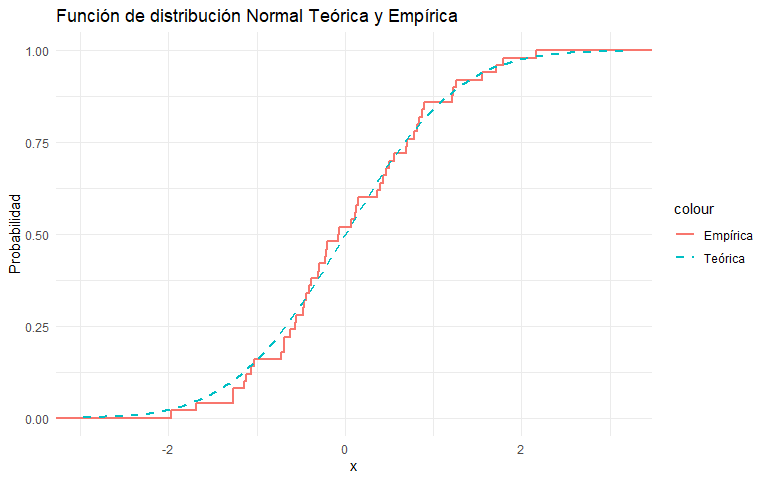
\includegraphics[width=\textwidth]{assets/TeoricaEmpirica.png}
    \caption{Visualización de una distribución teórica y empírica}
    \label{fig:theorical_vs_empirical}
\end{figure}

\subsection{Test Chi-Cuadrado de Bondad de Ajuste}

Sea $X_1,\dots,X_n$ con distribución F discreta:
\[
    \begin{matrix}
        C_1 \to P_1\\
        \dots \\
        C_k \to P_k
    \end{matrix}
    \quad
    p_j \geq 0,
    \quad \sum_{j=1}^{n} p_j=1
\]
Caso en el que $F_0$ completamente especificada bajo $H_0$:
\[
    H_0: p=p^0 \quad p=(p_1,\dots,p_k)'
\]
\[
    H_1: p \neq p^0 \quad p^0=(p_1^0,\dots,p_k^0)'
\]
Este problema ya lo sabemos resolver: es un contraste para el parámetro p de una distribución multinomial.

Frecuencia observada en $C_j: f_j=\sum_{i=1}^{n} \mathbbm{1}_{(x_i=c_j)}, \quad j=1,\dots,k \quad \sum_{j=1}^{k} f_j=n$

Frecuencia esperada bajo $H_0$ en $C_j$:
\[
    e_j=n \cdot P_0(x=c_j)=n \cdot p_j^0
\]

\textbf{Ejemplo:}

Sea una variable aleatoria $X$ cuya función de masa de probabilidad es la siguiente
\[
    P(X = x) = 
    \left\{
        \begin{matrix}
            \frac{1}{3} & \text{si } x = 0 \\[0.5em]
            \frac{1}{3} & \text{si } x = 1 \\[0.5em]
            \frac{1}{3} & \text{si } x = 2
        \end{matrix}
    \right.
\]

Entonces la hipotesis nula para el test será que

\[
    H_0:\quad p_1=\frac{1}{3} \quad p_2=\frac{1}{3} \quad p_3=\frac{1}{3}
\]

Tomando una muestra de n=10 quedan 7 ceros, 2 unos y 1 dos.

\vspace{5mm}

A simple vista no parece que siga esa distribución. Usaremos un estadístico para medir que tan diferente es de nuestra distribución pues lo que esperabamos obtener es:
\[
    \begin{matrix}
        e_1=3,33\\
        e_2=3,33\\
        e_3=3,33
    \end{matrix}
\]
El test $\chi^2$ de ajuste proporciona unas bases probabilisticas para decidir si las diferencias son suficientemente grandes tal que no hayan ocurrido por puro azar. Se define como
\[
    \chi^2=\sum_{j=1}^{k} \frac{(f_j-e_j)^2}{e_j}
\]
Este estadístico es lo que se conoce como distancia $\chi^2$ entre $f_j$ y $e_j$. Para valores grandes en $\chi^2$ implica frecuencias observadas y esperadas muy diferentes. 

\vspace{5mm}

\noindent Fijado $\alpha$:
\begin{itemize}
    \item Región critica: ($\chi^2 > C_\alpha$)
    \item p-valor: $p_0(\chi^2>X_{obs})=p_0(\chi^2>t_{obs})$
\end{itemize}

Necesitamos conocer la distribución del estadístico bajo $H_0$.
Se podría conocer de forma exacta aunque es muy complejo, por ello, nos interesará la distribución asintótica para $n$ grande.

\smallskip

\noindent \textbf{Resultado:}
\[
    \lim_{n \to \infty} P_0(\chi^2 \leq Z)=P(\chi^2_{k-1} \leq Z)
\]
La distribución asintótica del estadístico $\chi^2$ bajo $H_0$ es $\chi^2_{k-1}$ $g'$.

Ya hemos visto que en este contexto $ F_0 $ es una distribución multinomial. 
Vamos a ver que el estadístico $ T $ bajo $ H_0 $ para el modelo multinomial con $ k-1 $ parámetros libres es asintóticamente equivalente al estadístico $ \chi^2_1 $.

\begin{proofs}
    Estadístico RV para:
    \[
        H_0: F = F_0
    \]
    \[
        H_1: F \neq F_0
    \]
    Recordemos:
    \[
        L(p, x) = \prod_{j=1}^{k} p_j^{f_j} \quad \implies \quad \log L(p, x) = \sum_{j=1}^{k} f_j \log p_j
    \]
    El estadístico es:
    \[
        T = 2 \left[\log L(\widehat{p}, x) - \log L(p_0, x)\right] = 2 \left[ \sum_{j=1}^{k} f_j \log \widehat{p_j} - \sum_{j=1}^{k} f_j \log p_j^0 \right] 
    \]
    \[
        = -2 \sum_{j=1}^{k} \left( \log p_j^0 - \log \widehat{p_j} \right)
    \]
    Aproximamos $\log p_j^0$ por un desarrollo de Taylor en torno a $\log \widehat{p_j}$:
    \[
        \log p_j^0 \approx \log \widehat{p_j} + (p_j^0 - \widehat{p_j}) \frac{1}{\widehat{p_j}} - \frac{(p_j^0 - \widehat{p_j})^2}{2 \cdot \widehat{p_j}^2}+ \dots
    \]
    \[
        \to \log p_j^0- \log \widehat{p_j}\thickapprox (p^0_j-\widehat{p_j}) \frac{1}{\widehat{p_j}}- \frac{(p^0_j-\widehat{p_j})^2}{2}\frac{1}{\widehat{p_j^2}}
    \]
\end{proofs}

\newpage

\begin{proofs*}
    Sabiendo que $\widehat{p_j}=\frac{f_j}{n}$
    \[
        =\left(p_j^0-\frac{f_j}{n}\right) \cdot \frac{n}{f_j} - \frac{\left(p_j^0-\frac{f_j}{n}\right)^2}{2}\cdot \left(\frac{n}{f_j}\right)^2 \xrightarrow{c.s.} 0
    \]
    Esto converge a 0, ya que, por la Ley de los Grandes Números (LGN), $\frac{F_j}{n}$ es un estimador consistente de $p_j$:
    \[
        \lim_{n \to \infty} P \left( \left| \frac{F_j}{n} - p_j \right| > \varepsilon \right) = 0 \quad \forall \varepsilon>0
    \]
    Por lo tanto, el estadístico T queda:
    \[
        T = -2 \sum_{j=1}^{k} \left( n \cdot p_j^0 - f_j \right) + \frac{\sum_{j=1}^{k} (f_j - n \cdot p_j^0)^2}{f_j}
    \]
\end{proofs*}

El text $\chi^2$ y el TRV son asintóticamente equivalentes y como TRV converge a $\chi^2_{k-1}$, el estadístico $\chi^2$ también.
Fijado un $\alpha$.
\begin{itemize}
    \item Región critica: $P_0(\chi^2 \geq C_\alpha) \quad C_\alpha=qchisq(1-\alpha,k-1)$
    \item p-valor: $P_0(\chi^2 \geq t_{obs})=1-qchisq(t_{obs},k-1)$
\end{itemize}

\noindent \textit{Nota}:

Esta aproximación es válida para frecuencias mayores o iguales a 5

\vspace{5mm}

\textbf{Ejercicio 1}: Script R

\vspace{5mm}

\textbf{Ejercicio 4}: En una fábrica con 220 empleados, el número de trabajadores que tuvieron accidentes se recoge en latabla siguiente:

\begin{table}[!h]
    \centering
    \begin{tabular}{|c|c|c|c|c|c|c|c|}
        \hline
        {Nº accidentes} & 0 & 1 & 2 & 3 & 4 & 5 & 6+ \\ \hline
        {Nº trabajadores} & 181 & 9 & 4 & 10 & 7 & 4 & 5 \\ \hline
    \end{tabular}
\end{table}

¿Son estos datos consistentes con la distribución de Poisson con $\lambda=1$?

Tenemos una hipótesis compuesta ya que no conocemos el parámetro de la Poisson.
Si nos dijeran $P(1)$ sería simple.

\[
    f(x,1)=\frac{e^{-1}\cdot \lambda^x}{x!}=\frac{e^{-1}}{x!}
\]
\[
    p_0^0=e^{-1} ,\quad p_1^0=e^{-1} ,\quad p_2^0=\frac{e^-1}{2} ,\quad \dots,\quad p_6^0=1-\sum_{j=0}^{b}p_j^0
\]

Calculamos las frecuencias esperadas

\[
    e_0=220 \cdot e^{-1},\quad e_1=220 \cdot e^{-1}, \quad \dots
\]
\[
    \chi^2=\frac{(181-220 \cdot e^{-1})^2}{220 \cdot e^{-1}}+\dots
\]

Por tanto concluimos que es muy probable que no siga una P(1)

\textbf{Ejercicio 10:} Se lanza una moneda hasta que aparece la primera cara. Este experimento se repite 100 veces. LAs frecuencias observadas del numero de ensayos necesarios hasta que aparece la primera cara son:

\begin{table}[!h]
    \centering
    \begin{tabular}{|c|c|c|c|c|c|}
        \hline
        {Nº ensayos} & 1 & 2 & 3 & 4 & 5+ \\ \hline
        {Frecuencia} & 40 & 32 & 15 & 7 & 6 \\ \hline
    \end{tabular}
\end{table}

¿Se puede concluir que la moneda es perfecta?

Distribución geométrica:
\[
    P_p(X=k)=(1-p)^{k-1}p \quad o \quad P_p(X=k)=(1-p)^{k}p
\]
Probabilidad bajo $H_0$.
\[
    p_1^0=\frac{1}{2} \quad p_2^0=\frac{1}{2^2} \quad \dots \quad p_5=1-\sum_{k=1}^{4} p_k
\]

Como $H_0$ es ``Los datos provienen de una distribución geométrica $\left(\frac{1}{2}\right)$''.

Según el test, no rechazamos $H_0$.

Si en realidad los datos vienen de una distribución geométrica $\left(\frac{1}{3}\right)$,  
¿cuál es la probabilidad de que el test lo detecte?  
¿Y si vienen de una distribución geométrica $(0.52)$?

\subsection{Distribución del test bajo $H_1$}

Podemos aumentar la potencia sacrificando $\alpha$ o aumentando el tamaño de la muestra.  
Si queremos asegurar una potencia de, por ejemplo, $0.8$ o $0.9$, necesitamos calcular cuánto debe valer $n$.

Para esto, necesitamos conocer la distribución del test bajo $H_1$.

Resultado:
\[
\lim_{n \to \infty} P_{\theta_1} (\chi^2_{k-1} \leq t) = P(\chi^2_{k-1}(\delta) \leq t)
\]
Donde $\delta$ es el parámetro de descentralidad para la $\chi^2_{k-1}$ descentrada.

\textit{\textbf{Definición:}} La distribución asintótica bajo $H_1$ del estadístico $\chi^2$ de prueba de ajuste es una $\chi^2$ descentrada con $k-1$ grados de libertad y parámetro de descentralidad $\delta$.

La demostración no está incluida en este curso. Sin embargo, hacemos algunos comentarios sobre esta definición:

\textbf{Comentarios:} %Los comentarios eran formulajos y no me compilan
\begin{enumerate}
    \item   \begin{itemize}
        \item Si $X$ es una variable aleatoria tal que $X \sim N(0,1)$, entonces $X^2 \sim \chi^2_1$.
        \item Si $X_1, \dots, X_n$ son v.a.i.i.d. $N(0,1)$, entonces $\sum_{i=1}^{n} X_i^2 \sim \chi^2_n$.
        \item Si $X_1, \dots, X_n$ son v.a.i.i.d. $N(\mu, \sigma^2)$, entonces 
        $
        \sum_{i=1}^{n} \left( \frac{X_i}{\sigma} \right)^2 \sim \chi^2_n
        $
        descentrada con parámetro $\delta$.
    \end{itemize}
    \item Para contrastar 
    \[
    \begin{matrix}
        H_0: p_0 = (p_1^0, \dots, p_k^0) \\
        H_1: p \neq p^0
    \end{matrix}
    \]
    si bajo $H_1$ la alternativa 
    es $p = (p_1^1, \dots, p_k^1)$, el test $\chi^2$ sigue 
    una distribución $\chi^2_{k-1}(\delta)$, donde $\delta$ 
    mide la distancia entre los dos vectores:
    \[
    \Delta = \sum_{j=1}^{k} \frac{(p_j^1 - p_j^0)^2}{p_j^0}; \quad \delta = n \cdot \Delta
    \]
    O equivalentemente:
    \[
    \delta = \sum_{j=1}^{k} \frac{\left( n \cdot p_j^1 - n \cdot p_j^0 \right)^2}{n \cdot p_j^0}.
    \]
    \item Existen tablas para $\chi_{k-1}^{2'}(\delta)$ (por ejemplo, las tablas estándar de $\chi^2$ descentrada).
\end{enumerate}

\subsubsection*{Ejercicio 11:}  
Durante 60 meses consecutivos se observó la variable aleatoria X="nº de accidentes al mes en un cruce de carreteras". Los resultados fueron:

\begin{table}[!h]
    \centering
    \begin{tabular}{|c|c|c|c|c|}
        \hline
        {$X$} & 0 & 1 & 2 & 3+ \\ \hline
        {Nº de meses} & 23 & 18 & 12 & 7 \\ \hline
    \end{tabular}
\end{table}

\begin{enumerate}[label=\alph*)]
    \item Contrastar la hipótesis de que la distribución de X es geométrica:
    \[
        G(\theta);p_\theta(X=x)=\theta \cdot (1- \theta)^x, \quad X=0,1,2,\dots
    \]

    $H_0: X \sim G(\theta)=$EMV para $X \in \{0,1,2,3+\}$

    \[
        P_0^0=\theta, \quad P_1^0=\theta \cdot (1-\theta), \quad P_2^0=\theta \cdot (1-\theta)^2, \quad P_3^0=(1-\theta)^3
    \]
    \[
        L(\theta,f)=\prod_{j=1}^{4}[p_j^0]^{f_i}= \theta^{23}\cdot(\theta \cdot (1-\theta))^18 \cdot (\theta \cdot (1-\theta)^2)^12 \cdot ((1-\theta)^3)^7
    \]
    \[
        log L(\theta,f)=53 \log \theta+63 \log (1-\theta)
    \]
    \[
        \frac{d \log(\theta,f)}{d \theta}=\frac{53}{\theta}-\frac{63}{1-\theta} \Longrightarrow \widehat{\theta}=\frac{53}{53+63}
    \]
    Test $\chi^2$:
    \[
        \widehat{\chi^2}=\sum_{j=0}^{3} \frac{(f_j-60\cdot P_l^0(\widehat{\theta}))^2}{60 \cdot p_j^0(\widehat{\theta})} \sim \chi^2_2
    \]

    \item Potencia de $H_0:G(0.4) \quad B_n(2,0.6)$:
    \[
        P_1(\chi^2> C_{0.05})=P(\chi_3^2(\delta)>C_{0.05})
    \]
    \[
        S=n \cdot \Delta, \quad \Delta=\sum_{j=0}^{3} \left(\frac{(p_j^0-p_j^1)^2}{p_j^0}\right)
    \]
\end{enumerate}

\subsection{Test de Kolmogorov-Smirnov}
\subsubsection{Test de Kolmogorov-Smirnov para hipótesis simples}

$X_1,\dots, X_n$ i.i.d. con función de distribución F continua y se quiere contrastar
\[
    H_0: F=F_0 \quad H_1: F \neq F_0
\]

El test de Kolmogorov-Smirnov es más potente que el $\chi^2$ en el caso de F continua.
Tenemos:
\begin{itemize}
    \item $F_0 \to $ Función de distribución bajo $H_0$.
    \item $\widehat{F_n} \to$ Función de distribución muestral o empírica.
\end{itemize}
\[
    \widehat{F_n}(x)=\frac{1}{n} \sum_{i=1}^{n} \mathbbm{1}_{(x_i \leq x)}, \quad x \in \mathbb{R}
\]
Tambien se puede definir a partir de los estadísticos de orden:

\[
    \widehat{F_n}(x)=
    \left\{
    \begin{array}{ll}
        0, & \text{si} \quad x \leq X_{(1)}\\
        \frac{i}{n} & \text{si} \quad X_{(i)} \leq x \leq X_{(i+1)}, \quad i=1, \dots,n-1 \\
        1 & \text{si} \quad X_n \leq x
    \end{array}
    \right.
\]
\newpage

Propiedades:
\begin{enumerate}
    \item $n\cdot \widehat{F_n}(x)$ es el total de valores de la muestra menores o iguales a $x$ y sigue una distribución $B(n, F(x))$, $\forall x \in \mathbb{R}$
    \item Según el resultado anterior, junto con las propiedades de la distribución binomial, se tiene $\widehat{F}(x)$ es un estimador consistente de $F(x)$
    \[
        \lim_{n \to \infty} P(|\widehat{F_n}(x) - F(x)| < \varepsilon) \to 0
    \]
    \[
        \text{y es CAN: }\sqrt{n}\cdot(\widehat{F_n}(x)-F(x))\backsimeq N(0,F(x)(1-F(x)))
    \]
    \item Por el teorema de Glivenko-Cantelli, $\widehat{F_n}(x)$ converge uniformemente y casi seguro a $F(x)$.
\end{enumerate}

A medida que n crece, al función escalonada de $\widehat{F_n}(x)$ con saltos en los valores de los estadísticos de orden $X_{(1)},\dots,X_{(n)}$ aproxima la distribución $F(x)'$.  % Creo que eso no debería ser prima pero no soy un experto

Por lo tanto cuando n es grande, la mayor diferencia entre $\widehat{F_n}(x)$ y $F(x)$ converge a 0.

Este resultado nos sugiere el estadístico $D_n=sup_x[\widehat{F_n}(x)-F(x)]$ el cual es una medida razonable de la precisión de la estimación.

Llamaremos estadístico de Kolmogorov-Smirnov de una muestra a
\[
    D_n=sup_x|\widehat{F_n}(x)-F_0(x)|
\]
El test rechaza la hipótesis para valores grandes del estadísitico ($D_n>C$).
Como siempre debemos conocer la distribución de $D_n$ para obtener el valor crítico.

\begin{enumerate}
    \item Es importante ver que la máxima diferencia en $|\widehat{F_n}(x)-F_0(x)|$ es la máxima 
    diferencia en los puntos en los que $\widehat{F_n}(x)>F_0(x)$ y la máxima en los punto donde $F_0(x)>\widehat{F_n}(x)$. 
    Así podemos definir los estadísticos Kolmogorov-Smirnov de un lado.
    \[
        \left.\begin{matrix}
                D_n^+=sup_x(\widehat{F_n}(x)-F_0(x)) \\
                D_n^-=sup_x(F_0(x)-\widehat{F_n}(x))
        \end{matrix}\right\}
        D_n=max\{D_n^+,D_n^-\}
    \]
            
    $D_n^+$ y $D_n^-$ son útiles para conocer la distribución.

    \item La distribución de $D_n^+$, $D_n^-$ y $D_n$ no depende de $F_0$, es decir, $c_\alpha$ será el mismo sin importar si estamos contrastando diferentes hipótesis simples (Como por ejemplo $N(3,1)$, $exp(2)$, $\dots$). Se dice que el estadístivo es de distribución libre ya que no depende de $F_0$.
\end{enumerate}

\begin{figure}[h!]
    \centering
    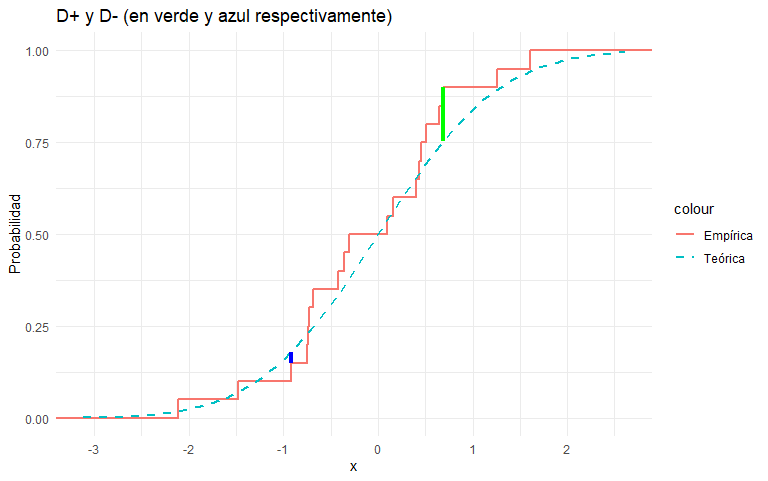
\includegraphics[width=\textwidth]{assets/Tema4/EjemploD.png}
    \caption{Visualización del estadísitico D+ y D-}
    \label{fig:Dplus_Dminus}
\end{figure}

Definimos los estadísticos de orden como $X_{(0)}=-\infty$ y $X_{(n)}=+\infty$, por lo tanto podemos definir $\widehat{F_n}(x)=\frac{i}{n} \quad \forall X_{(i)} \leq x < X_{(i+1)}$.

$D_n^+$ lo podemos ir calculando a trozos como:

\[
    D_n^+=sup_x(\widehat{F_n}(x)-F_0(x))
\]
    
Tomará un valor máximo unicamente en los extremos del intervalo $[X_{(i)},X_{(i+1)})$        
            
\[
    D_n^+=max_{1 \leq i \leq n}\left(\frac{i}{n}-F_0(x_{(i)})\right)
\]
Análogamente:
\[
    D_n^-=max_{1 \leq i \leq n}\left(F_0(x_{(i)})-\frac{i-1}{n}\right)
\]
$D_n^+,D_n^-$(por lo tanto $D_n$) dependen de las variables aleatorias.
\[
F_0(X_{(1)}),\dots,F_0(X_{(n)}) \sim U(0,1)
\]
Esto ocurre por la trasnformada integral de probabilidad, siempre y cuando las variables aleatorias sean continuas.

\subsubsection{Test de Kolmogorov-Smirnov para una hipótesis compuesta}

Lo anterior nos sirve para hipótesis simples. Sin embargo en la mayoría de los escenarios reales, tenemos hipótesis compuestas.
Por ejemplo, utlizar Kolmogorov-Smirnov en ANOVA.

Situación:
\[
H_0: F=F_0(\theta) \quad H_1:F \neq F_0(\theta)
\]
Lo haremos como siempre:
\begin{enumerate}
    \item Estimamos $\theta$ a partir de los datos(con el Estimador Máximo Verosimil).
    \item Se calcula el estadístico Kolmogorov-Smirnov como en el caso de la hipótesis simple:
    \[
        \widehat{D_n}=sup_x|\widehat{F_n}(x)-F(x)|
    \]
    Se rechaza $H_0$ con valores grandes de $\widehat{D_n}$ ($\widehat{D_n}>C$). 
    
    Es importante recalcar que $\widehat{D_n}$ no sigue la misma distribución que $D_n$.
    La distribución no es libre, depende de la familia que estemos evaluando.
\end{enumerate}

Tenemos tablas obtenidas por \href{https://es.wikipedia.org/wiki/Prueba_de_Lilliefors}{Lilliefors}
por simulación para la normal y para la exponencial.
Pasos a seguir:
\begin{enumerate}
    \item Se estiman los parámetros $\hat{\mu}$ y $\widehat{\lambda}$
    \item Se obtiene la muestra estandarizada $z_1,\dots,z_n$.
    \item Hacer el test ($H_0:F_0 \equiv N(0,1)$ en el caso normal y $H_0:F_0\equiv exp(1)$ en el caso exponencial).
    \item Se rechaza $H_0$ si $\widehat{D_n}>C$ para nivel $\alpha$. Se usan las tablas de \href{https://es.wikipedia.org/wiki/Prueba_de_Lilliefors}{Lilliefors}
    para definir $C_\alpha$.
\end{enumerate}

\textbf{Caso exponencial:}

\[
\begin{matrix}
    H_0:F \equiv exp(\lambda) \\
    H_1:F \not\equiv exp(\lambda)
\end{matrix}
\]
\[
    \widehat{\lambda}=\frac{1}{\bar{X}}, \quad z_i
    =\frac{X_i}{\bar{X}} \to z_i \sim exp(1)=\gamma(1,\lambda)
\]
El contraste es equivalente a:
\[
    H_0: X \sim \gamma\left(1,\frac{1}{\bar{X}}\right) \longleftrightarrow H_0:Z \sim \gamma(1,1)
\]

\vspace*{5mm}

\noindent Podrás descubrir más estadísticos en el campus virtual

\newpage
\section{Test de Shapiro-Wilk}
(Este test es más potente que el de Kolmogorov-Smirnov)

Mide como de bien se ajustan los datos a una distribución normal esperada. Se basa en combinación lineal de estadísticos ordenados. %Esto lo ha añadido en clase

\[
    W=\frac{\left(\sum_{i=1}^{n} a_i \cdot \chi_{(i)}\right)^2}{\sum_{i=1}^{n}(\chi_i-\bar{X})^2}
\]

donde

\begin{itemize}
    \item $\chi_{(i)} \longrightarrow$ estadístico de orden i.
    \item $a_i \longrightarrow$ coeficientes calculados a partir de los cuartiles esperados de una distribución normal estandar. 
\end{itemize}

\[
    (a_1,a_2,\dots,a_n)=\frac{m^T\cdot v^{-1}}{\sqrt{m^T \cdot V^{-1} \cdot V^{-1} \cdot m}}
\]

tal que

\begin{itemize}
    \item m=($m_{(1)},\dots,m_{(n)}$)
    \item V es la matriz de las covarianzas de $m_{(i)}$
\end{itemize}

El numerador nos indica como de bien se alinean los datos con la normalidad esperada. Si los datos son normales, el numerador será grande.

% ------------------------------------------------------------------------------

\newpage
\null

% ------------------------------------------------------------------------------

\begin{sectionpage}{Tema 5}{Contrastes basados en estadísticos de rangos}
    Introducción a los contrastes estadísticos basados en rangos para la comparación de muestras.
\end{sectionpage}

\subsection{Test de rangos}

Caso paramétrico normal.

$X_1,\dots,X_n$ i.i.d. $N(\mu_1,\sigma_1)$

$Y_1,\dots,Y_n$ i.i.d. $N(\mu_2,\sigma_2)$

\[
    H_0:\mu_1=\mu_2
\]
\[
    H_1: \mu_1 \neq \mu_2
\]

En el caso no paramétrico:

$X_1,\dots,X_n$ i.i.d. con distribución $F$

$Y_1,\dots,Y_n$ i.i.d. con distribución $G$

\[
    H_0:F=G
\]
\[
    H_1: F \neq G
\]

En ambos casos el objetico es el mismo, comparar tratamientos o resultados.

\textbf{Ejemplo:} 
Digamos que se quiere contrastar la eficacia de un nuevo medicamento para una enfermedad.
Lo primero que se tiene que hacer es diseñar un experimento para obtener los datos.

\begin{center}
    \href{https://media.tenor.com/lsbTX_Avt2AAAAAM/brushing-teeth-kowalski.gif}{Kowalski}, opciones (para diseñar el experimento xd):
\end{center}

\noindent Tenemos dos opciones...
\begin{enumerate}
    \item \textbf{Modelo de aleatorización}: Los datos vienen de un diseño controlado en el que los 
    individuos de análisis han sido asignados aleatoriamente a diferentes grupos.
    \item \textbf{Modelo poblacional:} Los datos son extraidos de una población y se asume que esa población tiene ciertas propiedades. 
    Por ejemplo: una distribución
\end{enumerate}

\subsubsection{Modelo de aleatorización}

Se dispone de $N$ individuos. Se eligen $n$ individuos a los que se asigna un tratamiento (una medición).
Caso donde

\[
    X_1,\dots,X_m \quad H_0: \text{El tratamiento no tiene efecto} 
\]
\[
    Y_1,\dots,Y_n \quad H_1: \text{El tratamiento tiene efecto} 
\]

El estadístico que utilicemos, rechazará $H_0$ cuando los valores de la variable considerada en los tratados sean mayores a los de control.
Para esto, usaremos \textbf{el estadístico basado en rangos}.
El estadístico basado en rangos, no depende de unidades de medida. Tomaremos toda la muestra y asignaremos rangos.

\textbf{\textit{Definición:}} Un rango es el lugar que ocupa la observación en la muestra ordenada.
Sean ($X_1,\dots,X_m$, $Y_1,\dots,Y_n$) nuestra muestra completa. Se ordenan los valores y se asignan rangos ($i_1,\dots,i_m,i_{m_1},i_n$)
Esto es la permutación donde $i_k$ es el valor que ocupa la observación k-ésima en la muestra ordenada.

\textbf{Ejemplo:}

Tenemos $X=\{5,8,9\}$ e $Y=\{6,7,10\}$

Por tanto la muestra completa será $\{5,8,9,6,7,10\}$

Que ordenado $\{5,6,7,8,9,10\}$, y se le asigna un rango a cada elemento ($\{1,2,3,4,5,6\}$)

\vspace{2mm}

\noindent \textit{Usando notación de tuplas, ($a, b$) donde $a$ es un elemento de la muestra y $b$ el rango asociado, la anterior asignación quedaría de la siguiente manera $\{(5, 1),(6, 2),(7, 3),(8, 4),(9, 5),(10, 6)\}$}

\vspace{2mm}

\noindent Por tanto quedarían asignados...

Rangos de $X$: $\{1,4,5\}$.

Rangos de $Y$: $\{2,3,6\}$.

\vspace{5mm}

\noindent \textbf{Notación formal:}

$R_1,\dots,R_m \longrightarrow$ rangos correspondientes a las observaciones $X_1,\dots,X_m$.

$S_1,\dots,S_n \longrightarrow$ rangos correspondientes a las observaciones $Y_1,\dots,Y_n$.

¿Cuando las $Y$ son mayores que las $X$?. Cuando $s_i$ sean más grandes, es decir, la suma de rangos sea más grande.

\paragraph{Estadístico de suma de rangos}

\textit{\textbf{Definición: }} La suma
\[
    W_s=s_1+\dots+s_n
\]
es conocida como \href{https://es.wikipedia.org/wiki/Prueba_de_los_rangos_con_signo_de_Wilcoxon}{el estadístico de Wilcoxon} de suma de rangos ($W_r=R_1+\dots+R_m$). Se rechazará $H_0$ para valores de $W_s$ grandes ($W_s>c_\alpha$).

\newpage

Como siempre, debemos conocer la distribución del estadístico de $W_s$ bajo $H_0$. Como la distribución es discreta, y podemos calcular lo siguiente...
\[
    P_{H_0}(W_s=k)=\sum_{s_1+\dots+s_n=k} P_{H_0} ((S_1,\dots,S_n)=(s_1,\dots,s_n))
\]

... encontrar la distribución de $W_s$ bajo $H_0$ se reduce a encontrar la distribución de ($S_1,\dots,S_n$).

\[
    P_{H_0} ((S_1,\dots,S_n)=(s_1,\dots,s_n))=\frac{1}{\binom{N}{n}}
\]
Cada resultado es igual de probable bajo $H_0$.


\textbf{Ejemplo:}
\noindent Dados $N=5$, $m=2$, $n=3$

\[
    \binom{N}{n}=\binom{5}{3}=\frac{5!}{3!\cdot2!}=10
\]
Habrá 10 posibles resultados de $s_1,s_2,s_3$.
\[
    \begin{array}{|c|c|c|c|c|c|}
    \hline
    \textbf{Tratados} & (1,2,3) & (1,2,4) & (1,2,5) & \dots & (3,4,5) \\ \hline
    P_{H_0}((S_1, \dots, S_n) = (s_1, \dots, s_n)) & 0.1 & 0.1 & 0.1 & \dots & 0.1 \\ \hline
    W_s & 6 &7 &8 & \dots &12 \\ \hline
    \end{array}
\]

\noindent Distribución de \(W_s\) bajo \(H_0\):
\[
    \begin{array}{|c|c|c|c|c|c|c|c|}
    \hline
    k & 6 & 7 & 8 & 9 & 10 & 11 & 12 \\ \hline
    P_{H_0}(W_s = k) & 0.1 & 0.1 & 0.2 & 0.2 & 0.2 & 0.1 & 0.1 \\ \hline
    \end{array}
\]

\noindent Rechazaremos $H_0$ cuando el valor de $W_s$ sea poco probable.

\vspace{2mm}

\noindent \textbf{Observaciones:}

La distribución de $W_s$ no es la misma si hubiéramos asignado $n$ a tratamientos y $m$ a control. Lo que es lo mismo, $W_R$ no sigue la misma distribución que $W_s$ bajo $H_0$. La distribución dependerá de n y m.

\subsubsection{Estadístico de Mann-Whitney}

En el caso anterior, el valor mínimo de $W_s$ corresponde a la situación a la que los individuos con tratamiento toman los valores más pequeños. Donde en el ejemplo anterior, $W_s=6 \quad 6=\frac{n \cdot (n+1)}{2}$.
Si consideramos el estadístico de Mann-Whitney,
\[
    W_{XY}=W_S-\frac{n(n+1)}{2}
\]
se nos facilitará hacer la tabla porque toma valores $0,1,\dots,(n \cdot m)$. Tomará el valor 0 cuando todos los valores de $Y$ son los más pequeños y el valor $n\cdot m$  cuando todos los $Y$ tomen los valores más grandes.

Una ventaja que tiene el estadístico es que toma los mismos valores sin importar la decisión de cuántos asignar a $n$ y cuántos a $m$.

Del mismo modo:
\[
    W_{YX}=W_R-\frac{m(m+1)}{2}
\]
$W_{YX}$ también toma valores 0,1,$\dots,n \cdot m$.

\noindent $W_{XY}$ y $W_{YX}$ siguen la misma distribución bajo $H_0$.

\noindent Existen tablas para esta distribución.

\vspace{2mm}

\noindent \textbf{Observaciones:}

La distribución bajo $H_0$ de $W_S$ (o $W_R)$ es simétrica respecto a $\frac{n \cdot (N+1)}{2}$.
\[
    \forall k \quad P_{H_0} \left( W_S=\frac{n \cdot (N+1)}{2}+k\right)=
    P_{H_0} \left( W_S=\frac{n \cdot (N+1)}{2}-k\right)
\]
Bajo $H_0$ $X$ e $Y$ están igualmente distribuidas, por lo que todos los elementos deberían ser indistinguibles en término de rangos. Por esto $W_{XY}$ y $W_{YX}$ están igualmente distribuidas bajo $H_0$.

\vspace{2mm}

\textbf{Ejemplo del uso de las tablas:}

\noindent Tenemos $W=10$, $n=6$, $m=4$

\noindent Queremos saber $P_{H_0}(W_s \geq 35)$

\noindent Tenemos las tablas para $W_{XY}=W_S-\frac{n \cdot (n+1)}{2}=W_S-21$

\noindent Debemos escribir $P_{H_0}(W_s \geq 35)$ como $P_{H_0}(W_{XY} \leq a)$

\noindent Sabemos que $W_S$ es simétrico a $\frac{n \cdot (N+1)}{2}=33$. Entonces...
\[
    P_{H_0}(W_S \geq 35)= P_{H_0}(W_S \geq 33+2)=P_{H_0}(W_S \leq 33-2)=P_{H_0}(W_S \leq 31)
\]
\[
    =P_{H_0}\left(W_S-\frac{n \cdot (n+1)}{2} \leq 31-21\right)= P_{H_0} (W_{XY} \leq 10)=0.3810 (\text{Usando las tablas})
\]
Llegaríamos al mismo resultado usando $W_S+W_R=55$.
\[
    P_{H_0}(W_S \geq 35)= P_{H_0}(W_R \leq 20)= P_{H_0} \left( W_R - \frac{m \cdot (m+1)}{2} \leq 20-10\right)
\]
\[
    = P_{H_0} (W_{YX} \leq 10)=0.3810
\]
Hay tablas hasta $n=m=10$. A partir de así usariamos la distribución asintótica.

\paragraph{Forma alternativa del estadístico de Mann-Whitney}

Una manera alternativa de ver el estadístico de Mann-Whitney que va a ser útil para calcular la potencia y también intervalos de confianza es la siguiente

\vspace*{2mm}

\textit{\textbf{Definición: }} Si $X_1,\dots,X_m$ son valores para individuos sin tratamientos y $Y_1,\dots,Y_n$ son valores para individuos con tratamiento,
y $W_{XY}=W_S-\frac{n \cdot (n+1)}{2}$, $W_{XY}$ es también el número de pares ($X_i,Y_j$) $i=1,\dots,m$, $j=1,\dots,n$ para los que $X_i < Y_i$
\[
    W_{XY}= \# [(X_i,Y_j) | X_i <Y_j]
\]

\begin{proofs}
    Sean $Y_{(1)}, \dots, Y_{(n)}$ valores ordenados de $Y_1,\dots,Y_n$ y sean $s_1,\dots,s_n$ los rangos correpondientes también ordenados,
    \begin{itemize}
        \item Hay $s_1-1$ observaciones menores que $Y_{(1)}$ y todas son $X$.
        \[
            \# [(X_i,Y_{(1)}) | X_i <Y_{(1)}]=S_1-1
        \]
        \item Hay $s_2-1$ observaciones menores que $Y_{(2)}$, de ellas una es $Y_{(1)}$ y el resto son $X$.
        \[
            \# [(X_i,Y_{(2)}) | X_i <Y_{(2)}]=S_2-1-1=S_2-2
        \]
        \item Hay $s_n-1$ observaciones menores que $Y_{(n)}$, de ellas $n-1$ son Y y el resto son $X$.
        \[
            \# [(X_i,Y_{(n)}) | X_i <Y_{(n)}]=S_n-n
        \]
    \end{itemize} 
    Por lo tanto:
    \[
        \# [(X_i,Y_j) | X_i <Y_j]=(S_1-1)+(S_2-2)+ \dots +(S_n-n)
    \]
    \[    
        =(S_1+\dots+S_n)-(1+2+\dots+n)=W_S-\frac{n \cdot (n+1)}{2}=W_{XY}
    \]
\end{proofs}

\vspace{5mm}

Distribución asintótica de $W_s$
Si los valores $n$ y $m$ son grandes (mayores que 10), se considera que la distribución asintótica para $W_S$ bajo $H_0$ es, por el Teorema Central del Limite...

\[
    \frac{W_S-E_0(W_S)}{\sqrt{Var_{0}(W_S)}} \xrightarrow[H_0]{L} N(0,1)
\]
\[
    E_0(W_S)=\frac{n \cdot (N+1)}{2} \quad Var_0(W_S)=\frac{n \cdot (N-n) \cdot (N+1)}{12}
\]
\subsection{Test de rangos con observaciones coincidentes}

Hemos visto contrastes para 2 muestras independientes, donde se eligen n individuos para un tratamiento y m para un grupo de control(u otro tratamiento), siendo N=n+m.
\begin{center}
    $H_0: $ Tratamiento no tiene efecto \\
    $H_1$ Tratamiento tiene efecto
\end{center}

Mediamos la variable de interés en los N individuos.
\begin{center}
    $X_1,\dots,X_m$ para los individuos de control \\
    $Y_1,\dots,Y_n$ para los individuos del tratamiento
\end{center}

Obteniamos los rangos de la muestra ($R_1,\dots,R_m$ y $S_1,\dots,S_n$).
Si la alternativa es mayor, se rechaza $H_0$ para $W_S=S_1+\dots+S_n>C$.
Si la alternativa es menor, se rechaza $H_0$ para $W_S=S_1+\dots+S_n<C$

¿Que pasa si hay coincidencias?

\newpage

\textbf{Ejemplo: }

Muestra:

\begin{center}
    1.2, 1.7, 1.7, 1.7, 2, 3.1, 3.1, 5
\end{center}

Los rangos serían:

\begin{center}
    1, 2, 2, 2, 5, 6, 6, 8
\end{center}

Pero estos rangos no serían correctos. Para aquellos valores en los que coincida el rango, se les dan distintos y el rango de todos los que coincidan se calculara como la media de sus rangos. Por tanto, los rangos serían:
1, 3, 3, 3, 5, 6.5, 6.5, 8

A esto lo vamos a llamar \textbf{semi-rangos}. Siempre que tengamos coincidencias, calcularemos los semi-rangos

\subsubsection{Semirangos}

\textbf{\textit{Definición: }}Los semi-rangos correspondientes a observaciones coinicidentes, se calculan como la media de los rangos que les corresponderían si no tuviéramos empates.

Notación:
Cuando haya coincidencias, los semi-rangos se asignan y representan como:
\begin{center}
$R_1^*,\dots,R_m^*$ semi-rango individual de control \\
$S_1^*,\dots,S_n^*$ semi-rango individual de tratamiento
\end{center}

Para controlar $H_0$, se rechaza si:
\[
    W_S^*=S_1^*+\dots+S_n^*>C
\]
Como siempre, necesitamos la distribución de $W_S^*$ bajo $H_0$ que no es la misma que cuando no hay coincidencias, aunque llegaremos a la distribución de la misma forma.

\textbf{Ejemplo:}
$n=m=3$

\(
X_1=5, \quad X_2=5, \quad X_3=9, \quad Y_1=5,\quad Y_2=10,\quad Y_3=10
\)

Los semi-rangos son 2,2,4 $\quad$ 2,5.5,5.5
(Nota: si los empates estan en el mismo grupo no nos afectan en nada)

\[
(S_1^*,S_2^*,S_3^*)=(2,5.5,5.5) \quad W_S^*=13
\]

Después de conocer los semi-rangos, calculamos la distribución de $W_S^*$ bajo $H_0$ de la misma forma que anteriormente.

Bajo $H_0$, (hipótesis de que el tratamiento no tiene efecto), los 6 individuos recibirían los semi-rangos independientemente de que fueran asignados al grupo de tratamiento o de control. Por lo tanto, para la selección de los 3 individuos a tratamiento, hay $\binom{6}{3}$
=20 posibles ekecciones de 3 individuos a tratamiento y 3 a control. Pero no todas diferentes, porque hay repetidos.

\begin{table}[h!]
    \centering
    \begin{tabular}{c|c|c|c|c|c|c}
    $S_1^*,S_2^*,S_3^*$ & $(2,2,2)$ & $(2,2,4)$ & $(2,2,5.5)$ & $(2,4,5.5)$ & $(2,5.5,5.5)$ & $(4,5.5,5.5)$ \\ \hline
    $W_S^*$             & $6$       & $8$       & $9.5$       & $11.5$      & $13$          & $15$          \\ \hline
    $P_{H_0}$           & $\frac{1}{20}$ & $\frac{3}{20}$ & $\frac{6}{20}$ & $\frac{6}{20}$ & $\frac{3}{20}$ & $\frac{1}{20}$
    \end{tabular}
\end{table}

La distribución depende de la configuración de las coincidencias. No se tienen tablas ya que habría que considerar cada caso.
Para n grande, se tiene al distribución asintótica bajo $H_0$.

\paragraph{Configuración de las coincidencias}

\textit{\textbf{Definición: }}Configuración de las coincidencias. 
\begin{itemize}
    \item Sea N=n+m el número de individuos tal que n sea el numero de individuos de control y m el numero de individuos del tratamiento
    \item Sea e el número de observaciones distintas entre los tratamientos
    \item Sea $d_1$, el número de observaciones iguales a la más pequeña
    \item Sea $d_2$, el número de observaciones iguales a la siguiente más pequeña
    \item Sea $d_e$ el número de observaciones iguales a la más grande
\end{itemize}

Al vector $(e,d_1,\dots,d_e)$ se le conoce como configuración de las coincidencias.

\textbf{Ejemplo}

$n=m=3$

\(
X_1=5, \quad, X_2=5, \quad X_3=9, \quad Y_1=5,\quad Y_2=10,\quad Y_3=10
\)

Los semi-rangos son 2,2,4;2,5.5,5.5

En este caso:
\[
    (e,d_1,\dots,d_e)=(3,3,1,2)
\]
\begin{itemize}
    \item El semirango de las $d_1$:
    \[
        \frac{1+\dots+d_1}{d_1}=\frac{d_1+1}{2}
    \]
    \item El semirango de las $d_2$:
    \[
        \frac{(d_1+1)+\dots+(d_1+d_2)}{d_2}=d_1+\frac{d_2+1}{2}
    \]
    \item El semirango i-ésimo
    \[
        \frac{(d_{i-1}+1)+\dots+(d_{i-1}+d_i)}{d_i}=d_1+\dots+d_{i-1}+\frac{d_i+1}{2}
    \]
\end{itemize}

\[
    d_1=\frac{3+1}{2}=2 \quad d_2=3+\frac{1+1}{2}=4 \quad d_3=3+1+\frac{2+1}{2}=5.5
\]

Estos conteos se pueden hacer solo para n y m pequeños. En este caso, podemos relacionar $W_S^*$ con el estadístico de Mann-Whitney análogo para el caso sin coincidencias.

\subsubsection{Estadístico de Mann-Whitney con observaciones no distintas}

El estadístico de $W_S^*$ es una generalización de $W_S$ cuando no todas las observaciones son distintas.
Del mismo modo, se puede generalizar el estadístico de Mann-Whitney. 

Sea $X_1,\dots,X_m$ valores de la variable de interés para control y $Y_1,\dots,Y_m$ valores de la variable de interés del tratamiento
,si todas las observaciones son distintas, definiamos el estadístico de Mann-Whitney como:
\[
    W_{XY}= \# [(X_i,Y_i)|X_i<Y_i]
\]
($\#$ = numero de casos en que: )

En caso de tener coincidencias, se puede definir para cada par $(X_i,Y_j)$
\[
    \phi(X_i,Y_j)=\left\{ 
        \begin{matrix}
            1 & si & X_i<Y_j \\
            \frac{1}{2} & si & X_i=Y_j \\
            0 & si & X_i>Y_j
        \end{matrix}
    \right.
\]

Si definimios $W_{XY}^*=\sum \phi (X_i,Y_j)$, es decir:

\[
    W_{XY}^* = \# [(X_i,Y_i)|X_i<Y_i] + \frac{1}{2} \cdot \# [(X_i,Y_i)|X_i=Y_i]
\]

Resultado: Los tests basados en $W_S^*$ y en $W_{XY}^*$ son equivalentes y además
\[
    W_{XY}^*=W_S^*-\frac{n \cdot (n+1)}{2}
\]

Demostración en el campus

\textit{Nota: se puede usar para categorías}

\paragraph{Distribución asintótica de $W_S^*$}

Si n y m son grandes y la proporción máxima de observaciones coincidentes no es próxima a 1, es decir, si:
\[
    max_{i=1,\dots,e}\left\{\frac{d_i}{N} \right\} << 1
\]

es decir, no hay un grupo en el que estén casi todas las observaciones.

\[
    \frac{W_S^*-E_\theta(W_S^*)}{\sqrt{Var_\theta(W_S^*)}} \xrightarrow{L} N(0,1)
\]
\[
    E_\theta(W_S^*)=\frac{n \cdot (N+1)}{2}
\]
\[
    Var_\theta(W_S^*)= \frac{n \cdot m \cdot (N-1)}{12}-n\cdot m \cdot \sum_{i=1}^{e} \frac{d_i \cdot (d_i^2-1)}{12-N \cdot (N+1)}
\]

\textbf{Ejercicio 9}
En un  estudio sobre la efectividad de los consejos psicológicos, 80 jovenes se dividen aleatoriamente en un grupo control de 40 jóvenes
, a quienes se aconseja de un modo tradicional, y un grupo de 40 que recibe un tratamiento especial. El cambio en el comportamiento de los jóvenes se califica como
pobre, medianamente pobre, medianamente bueno y bueno. Obtenemos los siguientes resultados:
\begin{table}[h!]
    \centering
    \begin{tabular}{|c|c|c|c|c|}
    \hline
    & Pobre & Medianamente pobre & Medianamente bueno & Bueno \\ \hline
    Tratamiento & 5 & 7 & 16 & 12 \\ \hline
    Control     & 7 & 9 & 15 & 9  \\ \hline
    \end{tabular}
\end{table}

Contrastar si el efecto del tratamiento es positivo.

Nos piden contrastar:

\begin{center}
    $H_0$: no hay diferencias entre control y tratamiento \\
    $H_1$: El tratamiento aumenta la respuesta
\end{center}

\newpage

Hay 4 grupos, por lo tanto e=4.

\begin{itemize}
    \item En el primer grupo hay 12 individuos
\end{itemize}

$(e,d_1,d_2,d_3,d_4)$=(4,12,16,31,21)

Semi-rangos:
\(
\left\{
\begin{matrix}
    d_1=\frac{12+1}{2}=6.5 \\
    d_2=12+\frac{16+1}{2}=20.5 \\
    d_3=12+16+\frac{31+1}{2}=44 \\
    d_4=12+16+31+\frac{21+1}{2}=70
\end{matrix}
\right.
\)

\[
    W_S^*=\sum_{i=1}^{4} B_i \text{(semirangos)}=5\cdot (65)+ 7\cdot (205)+ \dots+12 \cdot (70)=1720
\]

Vemos si el valor es grande con su distribución asintótica

El p-valor sería:
\[
    E_0(W_S^*) = \frac{n \cdot (N+1)}{2} = \frac{40 \cdot 81}{2} = 1620
\]
\[
    Var(W_S^*) = 9854.937
\]
\[
    P_{H_0}(W_S^* \geq 1720) = P \left( \frac{W_S^* - E(W_S^*)}{\sqrt{\text{Var}(W_S^*)}} \geq \frac{1720 - E(W_S^*)}{\sqrt{\text{Var}(W_S^*)}} \right)
\]
\[
    = P \left(Z \geq \frac{1720 - 1620}{\sqrt{9854.937}} \right) = 1 - \Phi(1.01) = 0.16
\]

\subsection{Modelo poblacional}

El precio que pagamos usando un modelo de aleatorización es que los resultados solo son válidos para los $N$ individuos de estudio y no se pueden extrapolar a una población más amplia.
Para que eso sea posible, será necesario que los $N$ individuos representen a toda la población. Dicho de otra forma, necesitamos una \textbf{muestra aleatoria simple} de la población.

La situación es la siguiente:
Tenemos $N=n+m$ individuos al azar de la población,

$$
\begin{aligned}
    n & \longrightarrow \text{elegidos al azar}\longrightarrow \text{grupo de tratamiento} \\
    m & \longrightarrow \text{restantes al grupo de control} \\
    \ & \ \\
    Y: & \text{ Variable respuesta de individuos que reciben el tratamiento}\\
    X: & \text{ Variable respuesta de individuos que son del grupo de control}  
\end{aligned}
$$

$X$ e $Y$ son dos variables aleatorias con funciones de distribución $X\sim F$ y $Y\sim G$ \\

\newpage

\noindent Queremos contrastar la hipótesis de que el tratamiento NO es efectivo

$$
\begin{aligned}
    H_0: & \text{ El tratamiento no tiene efecto }(F=G) \\
    H_1: & \text{ El tratamiento aumenta/disminuye la respuesta} (F>G/F<G)  
\end{aligned}
$$

El modelo poblacional tiene dos ventajas fundamentales:
\begin{enumerate}
    \item Los resultados son extrapolables
    \item Podemos estudiar la potencia del test
\end{enumerate}

\noindent Si tenemos un modelo poblacional sin coincidencias podemos utilizar el estadístico $W_s$ y el test de Wilcoxon $(W_s>C_\alpha)$; bajo $H_0$, $W_s$ sigue la misma distribución que en el modelo de aleatorización.

$$
\begin{aligned}
    X_1,\dots, X_m & \quad Y_1,\dots,Y_n\\
    R_1,\dots, R_m & \quad S_1,\dots,S_n
\end{aligned}
$$
$$
W_s=S_1+\dots+S_n
$$

Si hay coincidencias, tenemos que encontrar la distribución de $W^*_s$ bajo $H_0$. \\
En este caso el estadístico $W^*_s=S^*_1+\dots+S^*_n$ no es de distribución libre. La distribución bajo $H_0$ de los semi-rangos de los n individuos depende de F. 
Esto se debe (al igual que en el modelo de aleatorización) a que la distribución depende de la configuración de las coincidencias $(e,d_1,\dots,d_e)$, que en el modelo de aleatorización son un número pero aquí son variables aleatorias cuya distribución depende de F.\\

\hspace{-1cm}\noindent\begin{tabular}{r}
    \textbf{Ejemplo}  \\ \hline \ \\
\end{tabular}

    Supongamos $F$ discreta de tal forma que 
    
    $$
        F:\begin{cases}
            a & \text{Con probabilidad } p \\
            b & \text{Con probabilidad } 1-p
        \end{cases}
    $$
    Si $a<b$, y con $m=2$ y $n=1$, entonces los posibles resultados son:

    $$
    \begin{array}{c|c|c}
        X_1X_2Y_1 & \text{Probabilidad} & \text{Semi-rangos} \\ \hline
        a \; a \; a & p^3 & 2 \quad 2 \quad 2 \\ 
        a \; a \; b & p^2(1-p) & 1.5 \quad 1.5 \quad 2 \\ 
        a \; b \; a & p^2(1-p) & 1.5 \quad 2 \quad 1.5 \\ 
        b \; a \; a & p^2(1-p) & 2 \quad 1.5 \quad 1.5 \\ 
        a \; b \; b & p(1-p)^2 & 1 \quad 2 \quad 2 \\ 
        b \; b \; a & p(1-p)^2 & 2 \quad 2 \quad 1 \\ 
        b \; a \; b & p(1-p)^2 & 1.5 \quad 1 \quad 1.5 \\ 
        b \; b \; b & (1-p)^3 & 1 \quad 1 \quad 1 \\ 
    \end{array}
    $$
    La distribución de $W^*_s$ bajo $H_0$ será:

    $$
    \begin{array}{c|c c c c c}
        S^*_n & 1 & 1.5 & 2 & 2.5 & 3 \\ \hline 
        P_0(S^*_1=s^*_1) & p(1-p)^2 & 2p^2(1-p) & p^3+(1-p)^3 & 2p(1-p)^2 & p^2(1-p) \\
    \end{array}
    $$

Evidentemente la distribución de $W^*_s$ depende de p; es decir, de $F$.\\

Al igual que en el modelo de aleatorización, la distribución de $W^*_s$ depende de la configuración de las coincidencias, solo que esta vez esas coincidencias son v.a. que dependen de F.

\subsubsection{Potencia del test}
Una ventaja del modelo poblacional es que podemos calcular la potencia del test. Para ello debemos especificar la hipótesis alternativa. Sean $F$ y $G$ las distribuciones de las variables respuesta en individuos de control y tratamiento respectivamente,

$$
\begin{array}{c}
    H_0:\ F=G \\
    H_1:\text{ El tratamiento aumenta la respuesta, }F>G
\end{array}
$$

¿Qué significa en términos de $F$ y $G$ que el tratamiento aumente la respuesta?
$$
\forall z \in\mathbb{R}\quad\quad\quad P(Y>z)\geq P(X>z) \iff 1-G(z)\geq 1-F(z) \iff F(z)\geq G(z)
$$

\begin{theorem}
    Sean $X$ e $Y$ v.a. tales que $X\sim F$ y $Y\sim G$ con $F$ y $G$ funciones de distribución. Se dice que $Y$ (respecto a $X$) es estocásticamente mayor que $X$ (respecto a $Y$) cuando los valores que toma la v.a. $Y$ son mayores que los que toma la v.a. $X$, es decir:
    
    $$
    \begin{array}{c}
        G(z)\leq F(z)\quad\quad\quad\forall z \in\mathbb{R}\\
        H_0:\ F(x)=G(x)\\
        H_1:\ F(x)\geq G(x)
    \end{array}
    $$

\end{theorem}

El cálculo de la potencia requiere la distribución de los rangos. En el caso de F y G continuas es muy complicado, por lo que aproximaremos con la distribución asintótica y usaremos el estadístico de Mann-Whitney.

\paragraph{Potencia asintótica}

$$
\begin{array}{c}
    \Pi(F,G):\ X\sim F,\ Y\sim G\text{ si n y m son suficientemente grandes} \\
    \Pi(F,G)=\underset{\text{Bajo }H_1}{P_{F,G}}(W_{XY}\geq C_\alpha)=P_{F,G}\left(\frac{W_{XY}-E_{FG}(W_{XY})}{\sqrt{Var_{FG}(W_{XY})}}\geq \frac{C_\alpha-E_{FG}(W_{XY})}{\sqrt{Var_{FG}(W_{XY})}}\right)=\\
    =1-\Phi\left(\frac{C_\alpha-E_{FG}(W_{XY})}{\sqrt{Var_{FG}(W_{XY})}}\right)
\end{array}
$$

$$
\begin{array}{c}
    E(W_{XY})=mnp_1\\
    Var(W_{XY})=mnp_1(1-p_1)+mn(n-1)(p_2-p_1^2)+mn(m-1)(p_3-p_1^2)
\end{array}
$$

Siendo:

$$
\begin{array}{c}
    p_1=P_{FG}(X<Y)\\
    p_2=P(X<Y,X<Y')\\
    p_3=P(X<Y,X'<Y)
\end{array}
$$

El problema viene porque $p_1$, $p_2$ y $p_3$ son difíciles de calcular, por lo que usaremos una aproximación de la potencia.

\subsubsection{Modelo Shift de aproximación de la potencia}

\begin{theorem}
    $F$ y $G$ se agrupan en un modelo Shift si
    $$
    \exists\Delta>0,\ \forall x\quad\quad G(x)=F(x-\Delta)
    $$
\end{theorem}

El modelo Shift queda

$$
H_0:F(x)=G(x)\iff\Delta=0\quad\quad\quad H_1:G(x)=F(x-\Delta)\iff\Delta>0
$$

La potencia se escribe como:

$$
\Pi_F(\Delta)=P_\Delta(W_{XY}>C_\alpha),\ \Delta>0
$$
En particular, $\Pi_F(0)=\alpha$

\begin{theorem}
    Sea $F^*$ la función de distribución de la diferencia de las dos v.a. independientes con distribución F y sea $f^*(0)$ su densidad en el 0. Entonces
    $$
    \Pi(\Delta)\approx\Phi\left[\sqrt{\frac{12mn}{N+1}}f^*(0)\Delta-\mu_\alpha\right]
    $$
    Donde $\mu_\alpha\ /\ \Phi(\mu_\alpha)=1-\alpha$
\end{theorem}

Supongamos que $N$ es suficientemente grande como para poder usar la aproximación normal para encontrar $C_\alpha$

$$
\alpha = P_0(W_{XY}>C_\alpha)=P_0\left(\frac{W_{XY}-E_0(W_{XY})}{\sqrt{Var_0(W_{XY})}}\geq \frac{C_\alpha-E_0(W_{XY})}{\sqrt{Var_0(W_{XY})}}\right)
$$

$$
\begin{array}{c}
    W_{XY}=W_s-\frac{n(n+1)}{2}\\
    E(W_s)=\frac{n(N+1)}{2}\\
    E(W_{XY})=\frac{n(N+1)}{2}-\frac{n(n+1)}{2}=\dots=\frac{nm}{2}\\
    Var(W_{XY})=\frac{1}{12}mn(N+1)
\end{array}
$$

$$
\alpha=P_0\left(\frac{W_{XY}-\frac{1}{2}mn}{\sqrt{\frac{1}{12}mn(N+1)}}\geq \frac{C_\alpha-\frac{1}{2}mn}{\sqrt{\frac{1}{12}mn(N+1)}}\right)
$$

\newpage

Por lo que 

$$
\mu_\alpha=\frac{C_\alpha-\frac{1}{2}mn}{\sqrt{\frac{1}{12}mn(N+1)}} \Longrightarrow C_\alpha=\frac{1}{2}mn+\sqrt{\frac{1}{12}mn(N+1)}\mu_\alpha
$$

Calculando la potencia:

$$
    \Pi_F(\Delta)=P_\Delta\left(W_{XY}\geq\frac{1}{2}mn+\sqrt{\frac{1}{12}mn(N+1)}\mu_\alpha\right)=
$$
$$
    =P_\Delta\left(\frac{W_{XY}-E_\Delta(W_{XY})}{\sqrt(Var_\Delta(W_{XY}))}\geq\frac{\frac{1}{2}mn+\sqrt{\frac{1}{12}mn(N+1)}\mu_\alpha-mnp_1}{\sqrt{Var_\Delta(W_{XY})}} \right)=
$$
$$
    =1-\Phi\left(\frac{\left(\frac{1}{2}-p_1\right)mn+\mu_\alpha\sqrt{\frac{1}{12}mn(N+1)}}{\sqrt{Var_\Delta(W_{XY})}}\right)
$$

Sustituyendo $p_1=P_{FG}(X<Y)$

$$
    p_1=P_\Delta(X<Y)=P_0(X<Y-\Delta)=P_0(Y-X>\Delta)=P_0(\underbrace{Y-X}_\text{Misma dist. bajo $H_0$}-\Delta>0)=1-F^*(\Delta)
$$

$F^*(\Delta)$ será la función de distribución de la diferencia de las dos v.a. independientes con distribución F. Si desarrollamos $F^*(\Delta)$ en torno al 0 con el polinomio de Taylor, sabiendo que $(F^*(x))'=f^*(x)$ y por simetría respecto al 0:

$$
    F^*(\Delta)\approx F^*(0)+(\Delta-0) f^*(0)=\frac{1}{2}+\Delta f^*(0)
$$

Supongamos $D=X-Y$, $X\sim F$, $Y\sim F$ y $D\sim F^*$, entonces:

$$
    F^*(0)=P(D\leq 0)=P(X-Y\leq 0)=P(X\leq Y)=\frac{1}{2}
$$

Por lo tanto,

$$
    p_1=1-F^*(0)\approx\frac{1}{2}+\Delta f^*(0) \Longrightarrow p_1-\frac{1}{2}\approx \Delta f^*(0)
$$

Entonces, ya podemos hacer una primera aproximación para el cálculo de la potencia:

$$
    \Pi_F(\Delta)\approx \Phi\left(\frac{mn\Delta f^*(0)-\mu_\alpha\sqrt{\frac{1}{12}mn(N+1)}}{\sqrt{Var_\Delta(W_{XY})}}\right)
$$

Nos faltaría calcular $Var_\Delta(W_{XY})$. Podemos hallar una aproximación cuando $\Delta$ es pequeño, ya que 

$$
    Var_\Delta(W_{XY})\approx Var_0(W_{XY})=\frac{mn(N+1)}{12}
$$

\newpage

Por lo que la expresión para la potencia quedaría como

$$
    \Pi_F(\Delta)\approx\Phi\left(\frac{mn\Delta f^*(0)}{\sqrt{\frac{mn(N+1)}{12}}}-\mu_\alpha\right)=\Phi\left(\sqrt{\frac{12mn}{N+1}}\Delta f^*(0)-\mu_\alpha\right)
$$
\[
    =\Phi\left(\sqrt{\frac{12 \, m}{N+1}} \, \Phi^*(0) \Delta - \mu_\alpha\right) = \Pi
\]

\paragraph{Inverso}

\[
    \sqrt{\frac{12 \, m}{N+1}} \, \Phi^*(0) \Delta - \mu_\alpha = \Phi^{-1}(\Pi)
    \Longrightarrow 
    \frac{12 \, m}{N+1} = \frac{\left(\Phi^{-1}(\Pi) + \mu_\alpha\right)^2}{\left(\Phi^*(0) \Delta\right)^2}
\]

Aproximamos asumiendo $m \simeq  n$ y asumimos también $N$ suficientemente grande para que $N \simeq N+1$:
\[
    n \simeq \frac{\left(\Phi^*(0) \Delta + \mu_\alpha\right)^2}{6 \Delta^2 \Phi^*(0)^2}
\]

\paragraph{Intervalos de confianza para pares}

Calculamos diferencias de nuestros dos:
\[
    D_{ij} = Y_i - X_j \quad \text{para todas las pares } i=1, \dots, m \quad j=1, \dots, n
\]

Tomamos como estimador 
\(\hat{\Delta} = \text{mediana}(D_{ij})\) ya que la mediana es robusta y menos sesgada.

\paragraph{Test de signos para muestras pareadas}

Antes del tratamiento:
\[
    X = \{2, 4, 5, 6, 8\}
\]

Después del tratamiento:
\[
    Y = \{3, 5, 7, 4, 10\}
\]

Se calculan las diferencias:
\[
    D = \{3-2, 5-4, \dots\} = \{1, 1, 2, -2, 2\}
\]

Si no hubiera diferencias, se deberían distribuir las diferencias positivas y negativas (y viceversa). El estadístico:
\[
    S \sim b(n, 0.5)
\]

En un test bilateral, el $p$-valor:
\[
    p = 2 \cdot P(5 \leq \min(S^+, S^-))
\]


% ------------------------------------------------------------------------------

\begin{sectionpage}{Parcial 2024-2025}{Resolución e indicaciones}
    Resolución del examen parcial y recomendaciones para su preparación.
\end{sectionpage}

\section{Primer examen parcial}

\textbf{Ejercicio 1:}

Un artículo, producto de un tipo de componente mecánico que puede deteriorarse a dos velocidades distintas, depende de factores de fabricación no controlados.  
Se observa que el tiempo de vida ($X$) de cada componente sigue una mezcla de distribuciones exponenciales con las siguientes características:

\begin{itemize}
    \item Con probabilidad \(p\), el componente tiene un tiempo de vida \(X\) que sigue una distribución exponencial con parámetro \(\lambda_1\), lo cual corresponde a componentes con alta resistencia.
    \item Con probabilidad \(1-p\), el componente tiene un tiempo de vida \(X\) que sigue una distribución exponencial con parámetro \(\lambda_2\), lo cual corresponde a componentes con menor resistencia.
\end{itemize}

El fichero \texttt{Tiempos.RData} corresponde a un conjunto de observaciones independientes \(x_1, x_2, \dots \), que representan los tiempos de vida medidos en horas de varios componentes.

\begin{enumerate}
    \item Obtener el EMV y concretar su distribución asintótica para los parámetros del modelo que subyace a partir de estos datos.
    \textbf{Nota:} Planteadas las ecuaciones de verosimilitud, utilice la función \texttt{optim} para el cálculo del EMV.

    \[
    f(x, p, \lambda_1, \lambda_2) = p \cdot e^{-\lambda_1 x} + (1-p) \cdot e^{-\lambda_2 x}
    \]

    \[
    L(x, p, \lambda_1, \lambda_2) = \prod_{i=1}^{n} f(x_i, p, \lambda_1, \lambda_2) = \prod_{i=1}^{n} \left( p \cdot e^{-\lambda_1 x_i} + (1-p) \cdot e^{-\lambda_2 x_i} \right)
    \]

    \[
    \log L(x, p, \lambda_1, \lambda_2) = \sum_{i=1}^{n} \log f(x_i, p, \lambda_1, \lambda_2)
    \]

    \[
    \begin{pmatrix}
        \widehat{p} \\
        \widehat{\lambda}_1 \\
        \widehat{\lambda}_2
    \end{pmatrix}
    \sim
    N_3
    \left(
    \begin{pmatrix}
        p \\
        \lambda_1 \\
        \lambda_2
    \end{pmatrix},
    \text{Var}(\text{EMV})_{3 \times 3}
    \right)
    \]

    \item Obtener el IC de Wald con confianza aproximada de \(95\%\) para cada parámetro del modelo.

    \[
    \widehat{p} \pm \texttt{qnorm}(0.975) \cdot \sqrt{\text{Var}(\widehat{p})}
    \]

    \item Obtener el \textit{p-valor} basado en el estadístico de Wald para contrastar la hipótesis \(H_0: \lambda_1 = 0.5\) vs. \(H_a: \lambda_1 \neq 0.5\).

    \[
    W = \frac{(\widehat{\lambda}_1 - 0.5)^2}{\text{Var}(\widehat{\lambda}_1)} \sim \chi^2_1
    \]

    \item Obtener el \textit{p-valor} basado en el estadístico de RV para contrastar la hipótesis \(H_0: \lambda_1 = 0.5\) vs. \(H_a: \lambda_1 \neq 0.5\).

    \[
    Q_L = 2 \cdot \left[ \log L(\widehat{p}, \widehat{\lambda}_1, \widehat{\lambda}_2, x) - \sup_{p, \lambda_2} \log L(p, \lambda_1 = 0.5, \lambda_2, x) \right] \sim \chi^2_1
    \]

\end{enumerate}


% ------------------------------------------------------------------------------

\newpage

% ------------------------------------------------------------------------------
% Reference and Cited Works
% ------------------------------------------------------------------------------

\begin{thebibliography}{9}
    \bibitem{manuscritos1}
    Juan Camilo Yepes Borrero, \\ \textit{Apuntes Manuscritos Tema 1}. \\ Universidad de Valladolid 2024.
    \bibitem{apuntes1}
    Yolanda Larriba González, \\ \textit{Apuntes INFE2 Tema 1}. \\ Universidad de Valladolid 2023.
    \bibitem{manuscritos2}
    Juan Camilo Yepes Borrero, \\ \textit{Apuntes Manuscritos Tema 2}. \\ Universidad de Valladolid 2024.
    \bibitem{apuntes2}
    Yolanda Larriba González, \\ \textit{Apuntes INFE2 Tema 2}. \\ Universidad de Valladolid 2023.
    \bibitem{manuscritos4}
    Juan Camilo Yepes Borrero, \\ \textit{Apuntes Manuscritos Tema 4}. \\ Universidad de Valladolid 2024.
    \bibitem{apuntes4}
    Yolanda Larriba González, \\ \textit{Apuntes INFE2 Tema 4}. \\ Universidad de Valladolid 2023.
    \bibitem{manuscritos5}
    Juan Camilo Yepes Borrero, \\ \textit{Apuntes Manuscritos Tema 5}. \\ Universidad de Valladolid 2024.
    \bibitem{apuntes5}
    Yolanda Larriba González, \\ \textit{Apuntes INFE2 Tema 5}. \\ Universidad de Valladolid 2023.
    \bibitem{examen}
    Juan Camilo Yepes Borrero, \\ \textit{Resolución examen en el aula}. \\ Universidad de Valladolid 2024.
\end{thebibliography}

% ------------------------------------------------------------------------------

\end{document}

